%%%%%%%%%%%%%%%%%%%%%%%%%%%%%%%%%%%%%%%%%%  不使用 authblk 包制作标题  %%%%%%%%%%%%%%%%%%%%%%%%%%%%%%%%%%%%%%%%%%%%%%
%-------------------------------PPT Title-------------------------------------
\title{\rm{VASP}的并行、迭代算法和赝势}
%-----------------------------------------------------------------------------

%----------------------------Author & Date------------------------------------
\author[\textrm{Jun\_Jiang}]{姜\;\;骏\inst{}} %[]{} (optional, use only with lots of authors)
%% - Give the names in the same order as the appear in the paper.
%% - Use the \inst{?} command only if the authors have different
%%   affiliation.
\institute[BCC]{\inst{}%
%\institute[Gain~Strong]{\inst{}%
\vskip -20pt 北京市计算中心}
%\vskip -20pt {\large 格致斯创~科技}}
\date[\today] % (optional, should be abbreviation of conference name)
{	{\fontsize{6.2pt}{4.2pt}\selectfont{\textcolor{blue}{E-mail:~}\url{jiangjun@bcc.ac.cn}}}
\vskip 45 pt {\fontsize{8.2pt}{6.2pt}\selectfont{%清华大学\;\;物理系% 报告地点
	\vskip 5 pt \textrm{2023.04.21}}}
}

%% - Either use conference name or its abbreviation
%% - Not really information to the audience, more for people (including
%%   yourself) who are reading the slides onlin%%   yourself) who are reading the slides onlin%%   yourself) who are reading the slides onlineee
%%%%%%%%%%%%%%%%%%%%%%%%%%%%%%%%%%%%%%%%%%%%%%%%%%%%%%%%%%%%%%%%%%%%%%%%%%%%%%%%%%%%%%%%%%%%%%%%%%%%%%%%%%%%%%%%%%%%%

\subject{}
% This is only inserted into the PDF information catalog. Can be left
% out.
%\maketitle
\frame
{
%	\frametitle{\fontsize{9.5pt}{5.2pt}\selectfont{\textcolor{orange}{“高通量并发式材料计算算法与软件”年度检查}}}
\titlepage
}
%-----------------------------------------------------------------------------

%------------------------------------------------------------------------------列出全文 outline ---------------------------------------------------------------------------------
\section*{}
\frame[allowframebreaks]
{
  \frametitle{Outline}
%  \frametitle{\textcolor{mycolor}{\secname}}
  \tableofcontents%[current,currentsection,currentsubsection]
}
%%在每个section之前列出全部Outline
%%类似的在每个subsection之前列出全部Outline是\AtBeginSubsection[]
%\AtBeginSection[]
%{
%  \frame<handout:0>%[allowframebreaks]
%  {
%    \frametitle{Outline}
%%全部Outline中,本部分加亮
%    \tableofcontents[current,currentsection]
%  }
%}

%-----------------------------------------------PPT main Body------------------------------------------------------------------------------------
\small
\section{\rm{VASP}软件}
\frame
{
	\frametitle{\textrm{VASP}软件简介}
	\textrm{VASP}软件是维也纳大学\textrm{(Universit\"at Wien)}~\textrm{G. Kresse}等开发的第一原理模拟软件包
	\begin{itemize}
		\item \textrm{VASP}采用\textrm{PAW~(Projector Augmented-Wave)}方法\upcite{PRB50-17953_1994,PRB59-1758_1999},平衡了赝势方法和全电子计算优点,兼顾了计算的精度和效率
		\item \textrm{VASP}在实空间优化投影函数\textrm{(Projector)},将主要的计算过程变换到实空间完成,大大节省了内存的开销%,保证了计算精度和效率
		\item \textrm{VASP}通过引入多样的优化算法,提高了矩阵对角化和电荷密度搜索的效率\upcite{CMS6-15_1996,PRB54-11169_1996}
		\item 在\textrm{VASP}的并行计算中,有效均衡了各节点处理\textrm{FFT}变换负载和通信,提升了软件的并行效率
	\end{itemize}
	相比于其他第一原理计算软件,\textrm{VASP}从物理思想与方法、优化算法和并行计算实现等多个方面都有更为出色的性能\upcite{PRL55-2471_1985,PRB47-10142_1993}
}

\frame
{
	\frametitle{\textrm{VASP}的开发团队}
\begin{figure}[h!]
\centering
\vspace*{-0.25in}
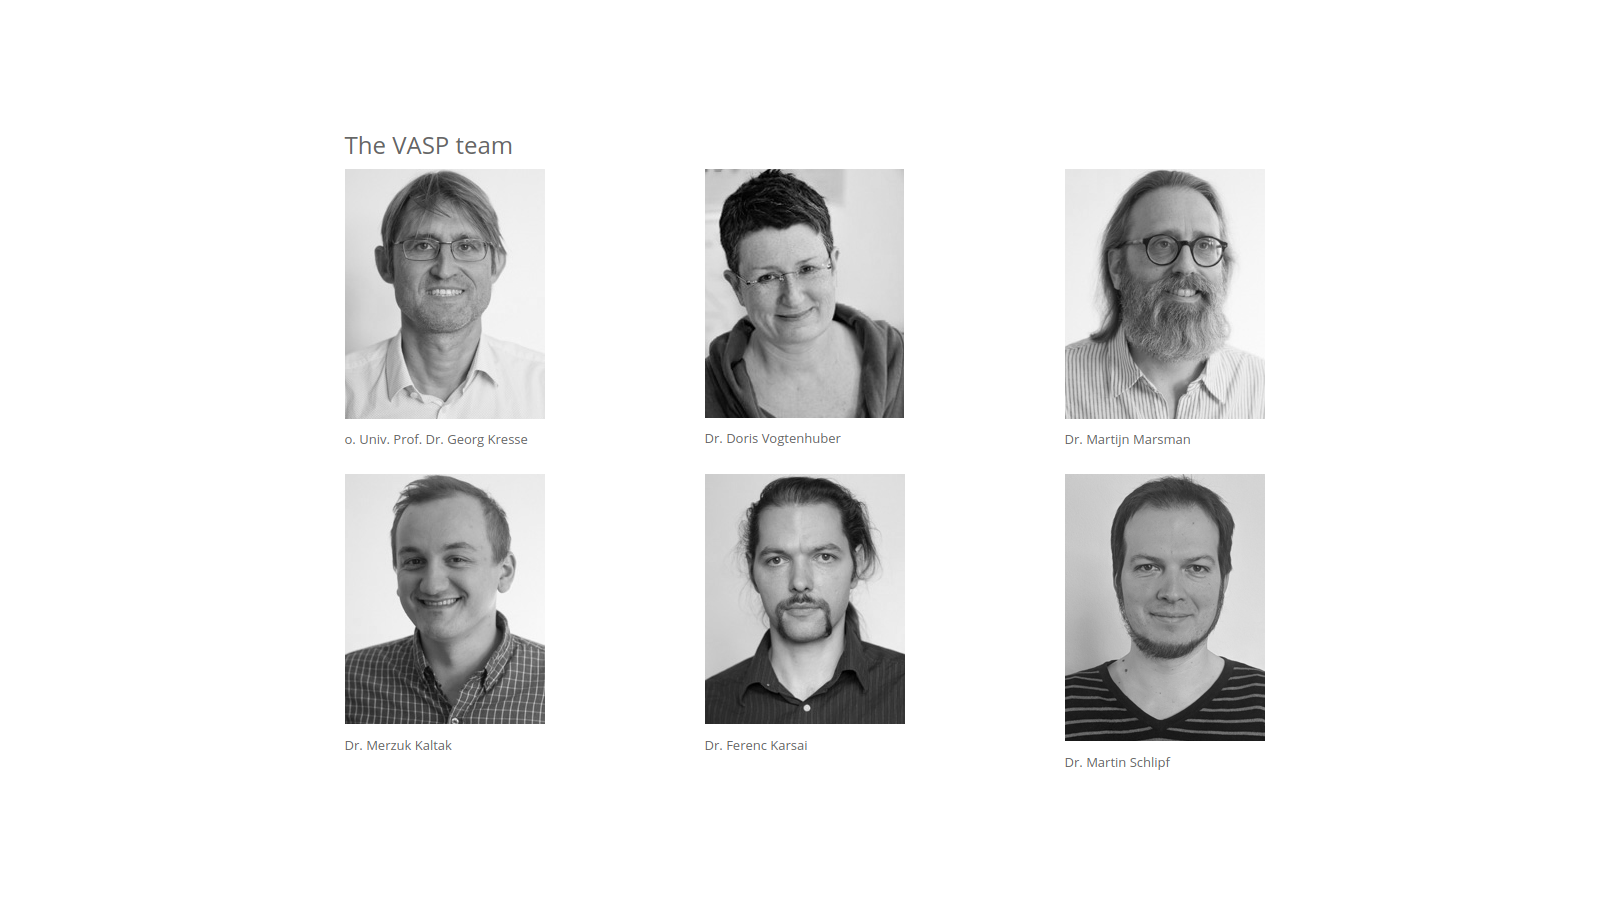
\includegraphics[height=2.70in,width=4.05in,viewport=330 130 1280 770,clip]{Figures/VASP_team.png}
\caption{\tiny \textrm{The development team of VASP.}}%(与文献\cite{EPJB33-47_2003}图1对比)
\label{VASP_team}
\end{figure}
}

\frame
{
	\frametitle{\textrm{VASP}的\textrm{Kohn-Sham}方程求解流程}
\begin{figure}[h!]
	\vspace{-0.2in}
\centering
%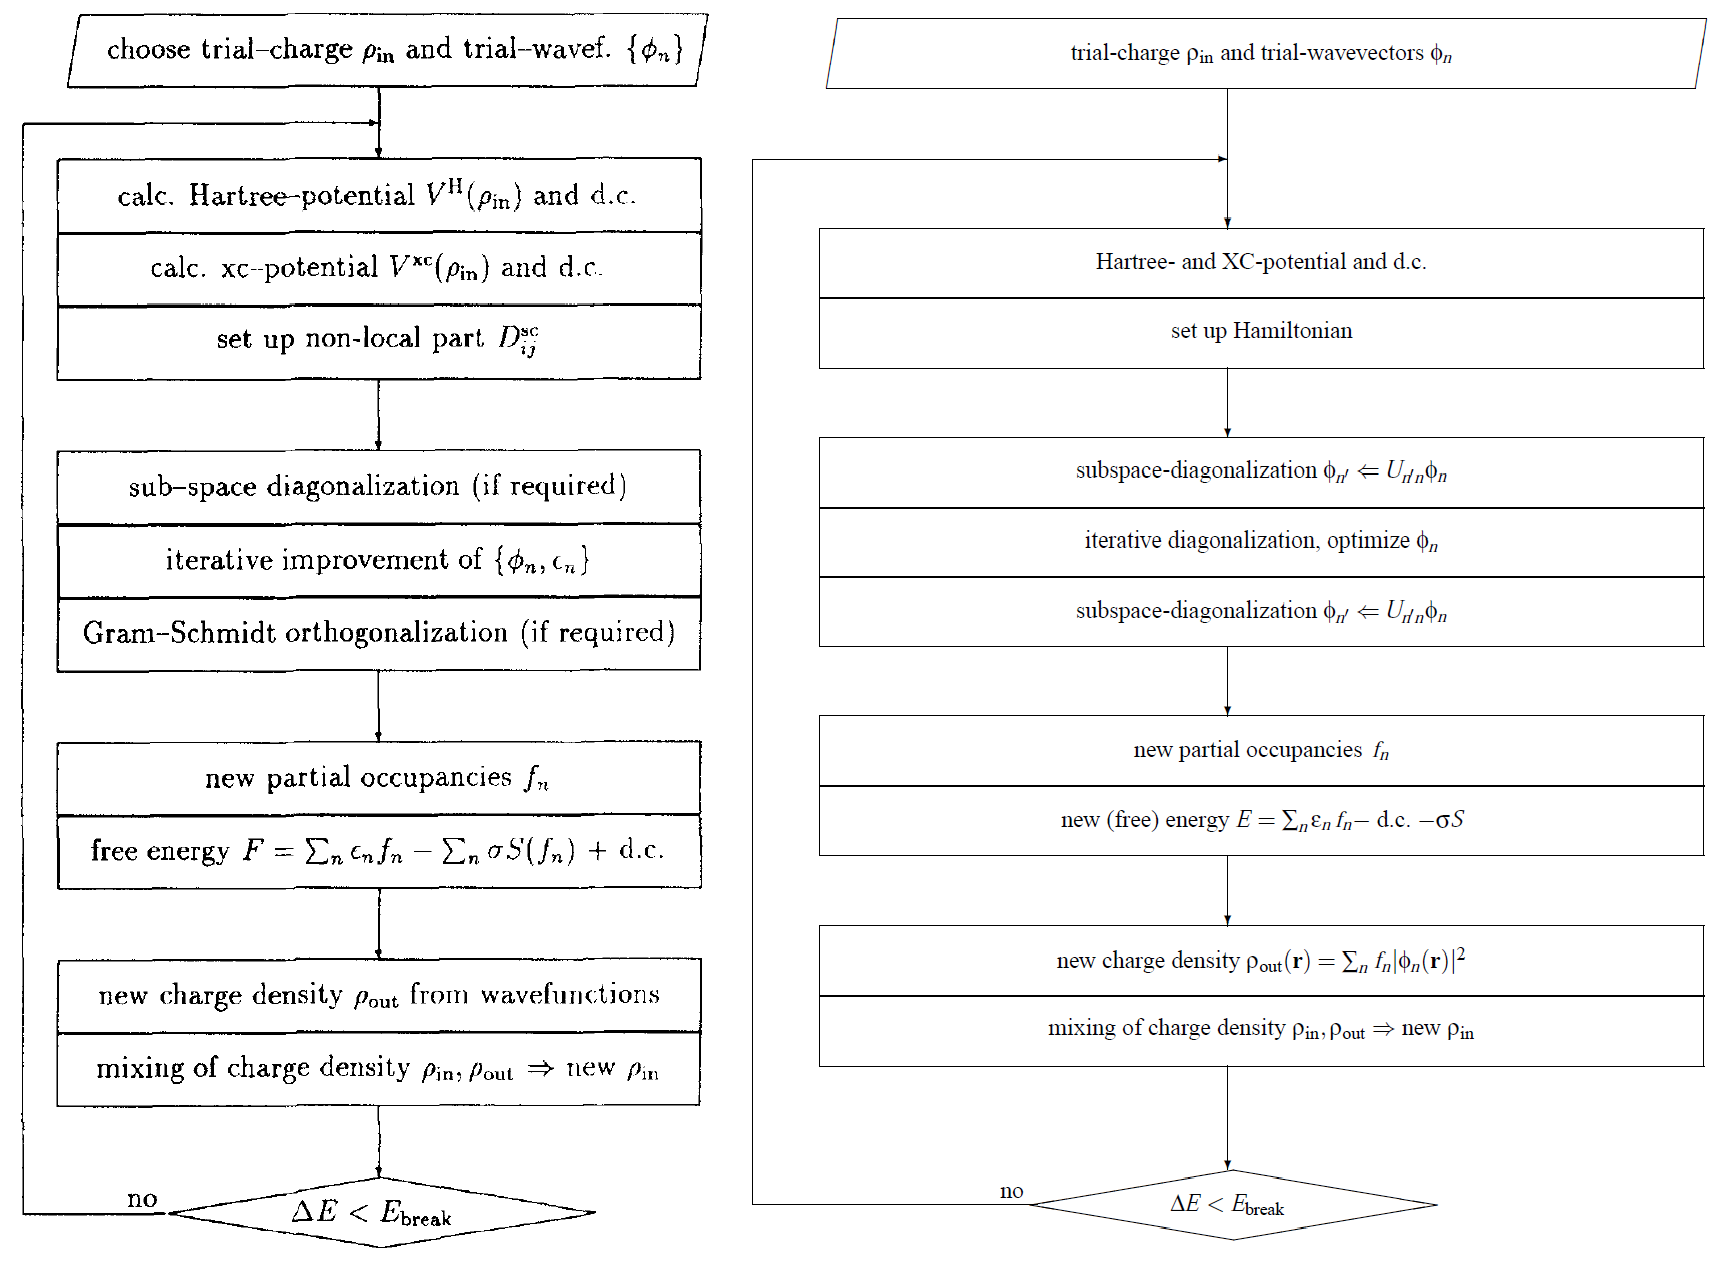
\includegraphics[height=2.7in,width=4.0in,viewport=0 0 1300 960,clip]{Figures/VASP_procedure-full.png}
%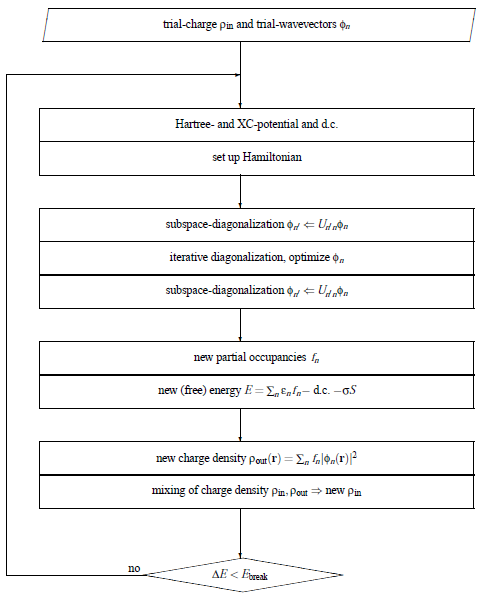
\includegraphics[height=2.1in,width=1.6in,viewport=0 0 480 630,clip]{Figures/VASP_procedure.png}
%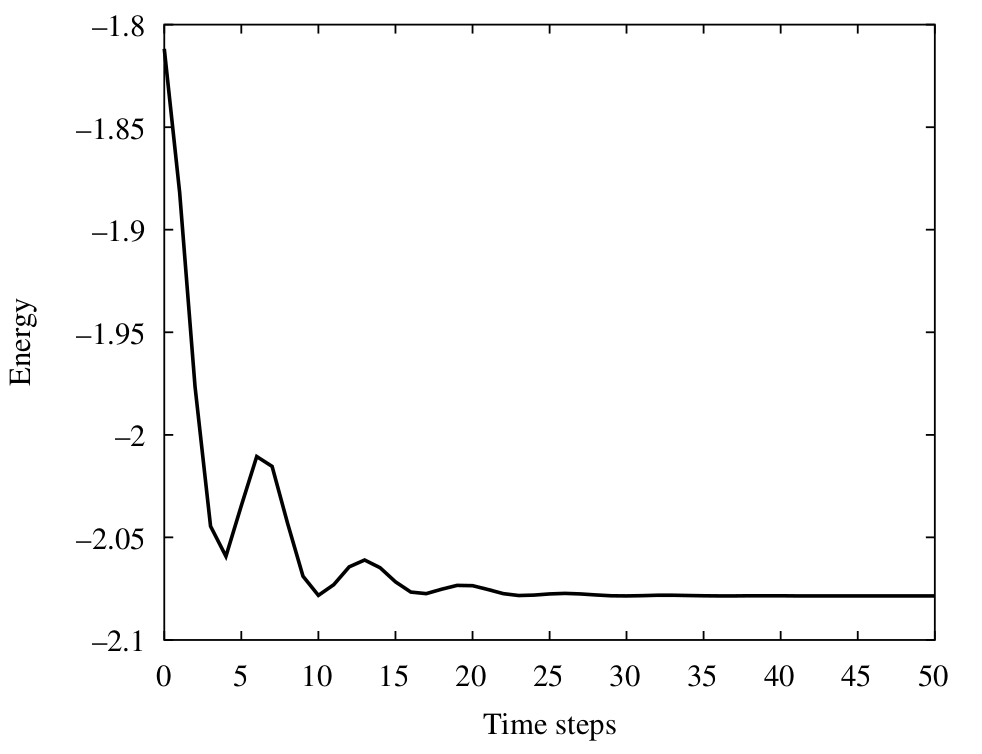
\includegraphics[height=2.1in,width=2.3in,viewport=0 0 740 600,clip]{Figures/Ab-initio-Ene.png}
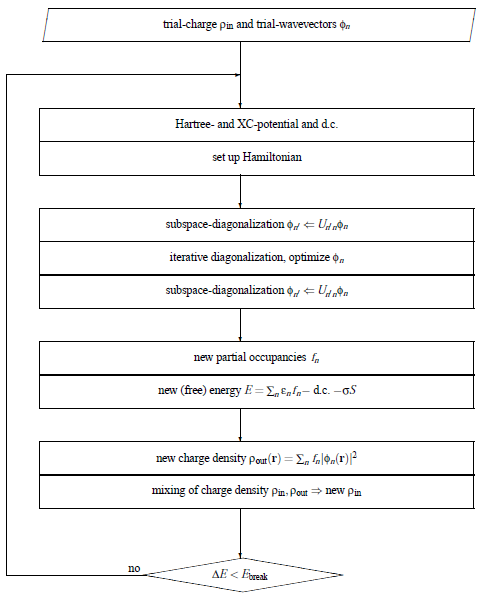
\includegraphics[height=2.75in,width=2.5in,viewport=0 0 480 630,clip]{Figures/VASP_procedure.png}
\caption{\tiny \textrm{The Flow of calculation for the KS-ground states.}}%(与文献\cite{EPJB33-47_2003}图1对比)
\label{PAW_baiseset}
\end{figure} 
}

\frame
{
	\frametitle{双网格技术}
\begin{figure}[h!]
	\vspace{-0.15in}
\centering
%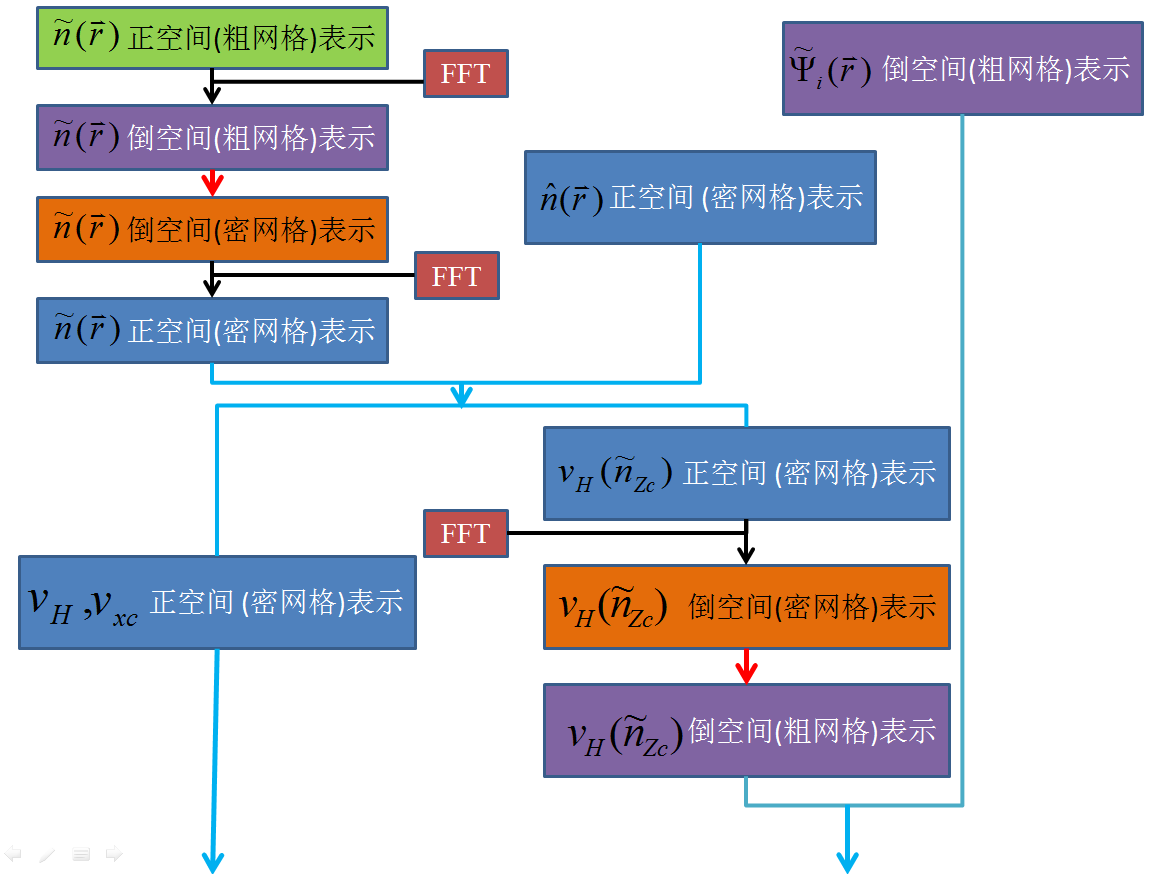
\includegraphics[height=2.7in,width=4.0in,viewport=0 0 1180 875,clip]{Figures/dual_grid.png}
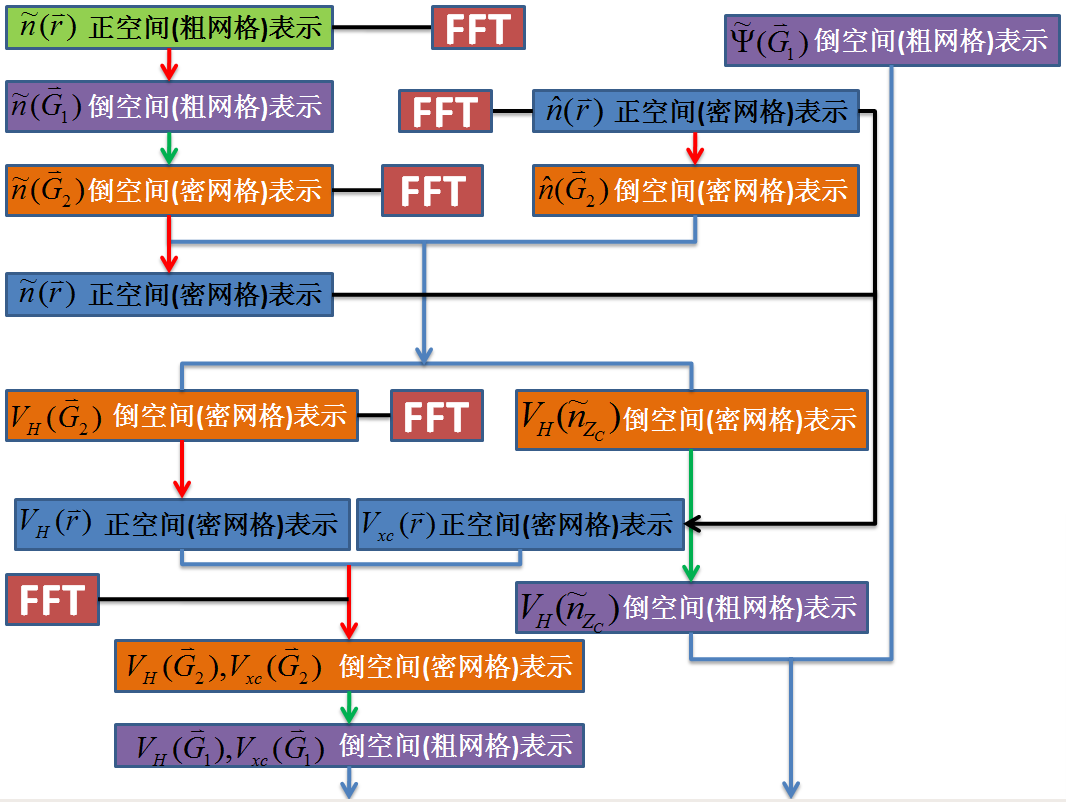
\includegraphics[height=2.75in,width=4.0in,viewport=0 0 800 600,clip]{Figures/dual_grid-2.png}
\caption{\tiny \textrm{The Schematic description of the dual grid technique.}}%(与文献\cite{EPJB33-47_2003}图1对比)
\label{PAW_dualgrid}
\end{figure} 
}

\frame
{
	\frametitle{\textrm{VASP}的并行效率}
	与同类型软件相比,\textrm{VASP}有着优异的并行能力
\begin{figure}[h!]
	\vspace{-0.15in}
\centering
%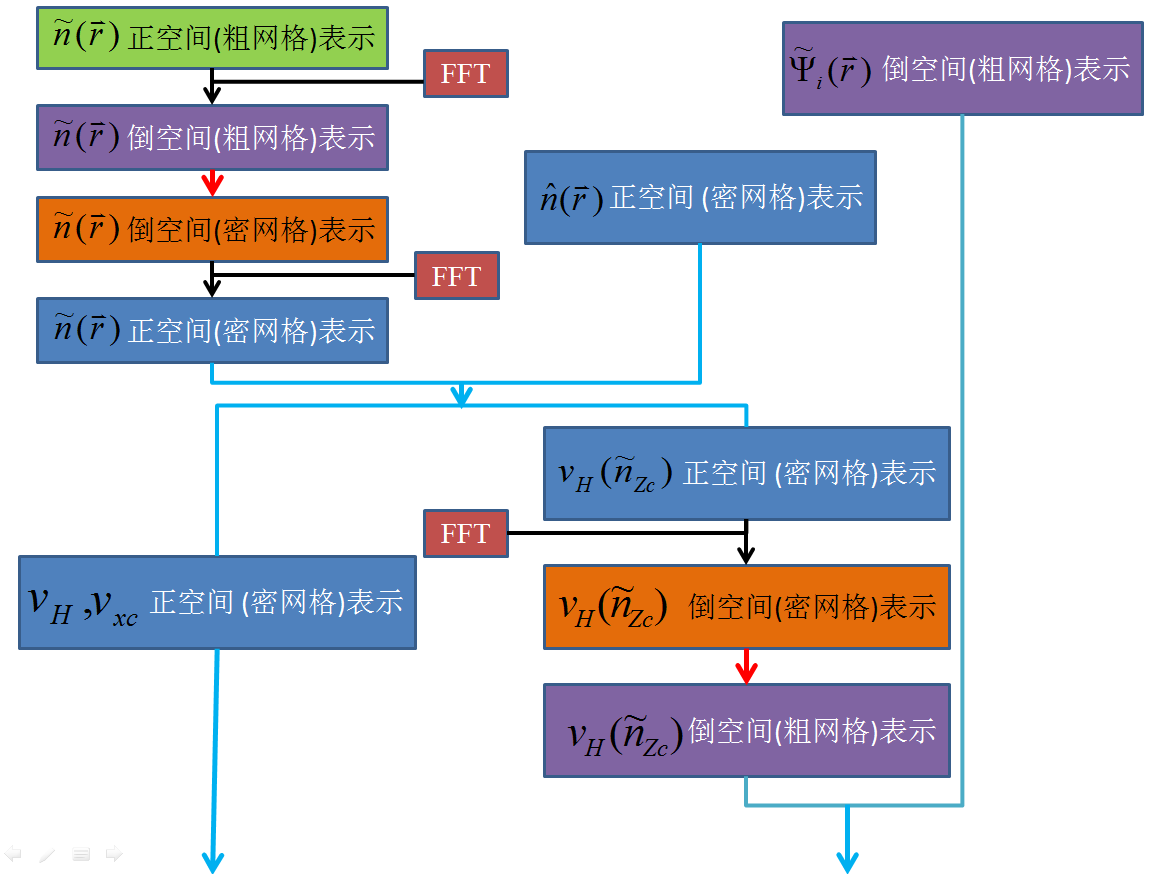
\includegraphics[height=2.7in,width=4.0in,viewport=0 0 1180 875,clip]{Figures/dual_grid.png}
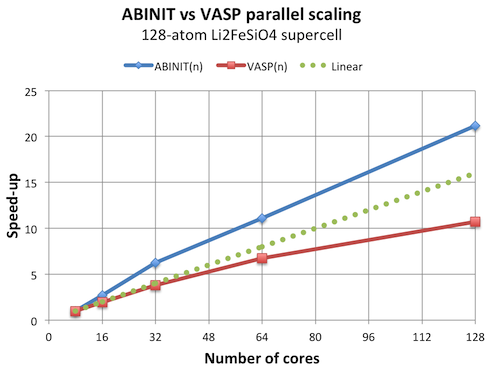
\includegraphics[height=1.55in,width=1.95in,viewport=0 0 240 200,clip]{Figures/VASP-abinit_Li128-1.png}
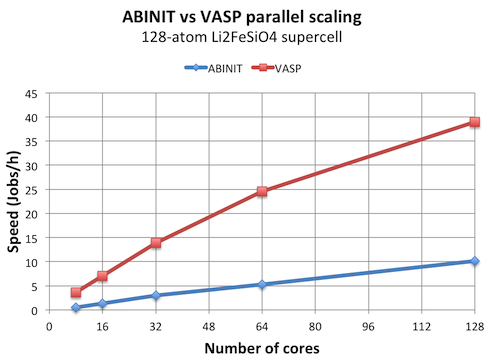
\includegraphics[height=1.55in,width=1.95in,viewport=0 0 240 200,clip]{Figures/VASP-abinit_Li128-2.png}
\caption{\tiny \textrm{The comparison of parallel scaling for ABINIT vs VASP.}}%(与文献\cite{EPJB33-47_2003}图1对比)
\label{ABINIT_vs_VASP}
\end{figure} 
\begin{itemize}
	\item \textrm{VASP}迭代对角化约束了矩阵的维度,减少了对角化过程中的迭代次数,保证了\textrm{MPI}并行的规模和扩展性
	\item \textrm{VASP}实施\textrm{FFT}变换时,保证各节点上处理的网格负载均衡
\end{itemize}
}

\frame
{
	\frametitle{\textrm{VASP}计算的\textrm{FFT}并行实现}
	\begin{itemize}
	     \item 中间层设计:~\textrm{FFT}网格、实空间基组与计算节点的匹配\\
		     \textcolor{red}{通过子程序\textrm{mgrid.F}生成中间层,实现并行负载与计算节点分配的匹配,减少\textrm{FFT}变换和实空间并行的节点间通信}
\begin{figure}[h!]
		\vspace{-0.25in}
	\centering
%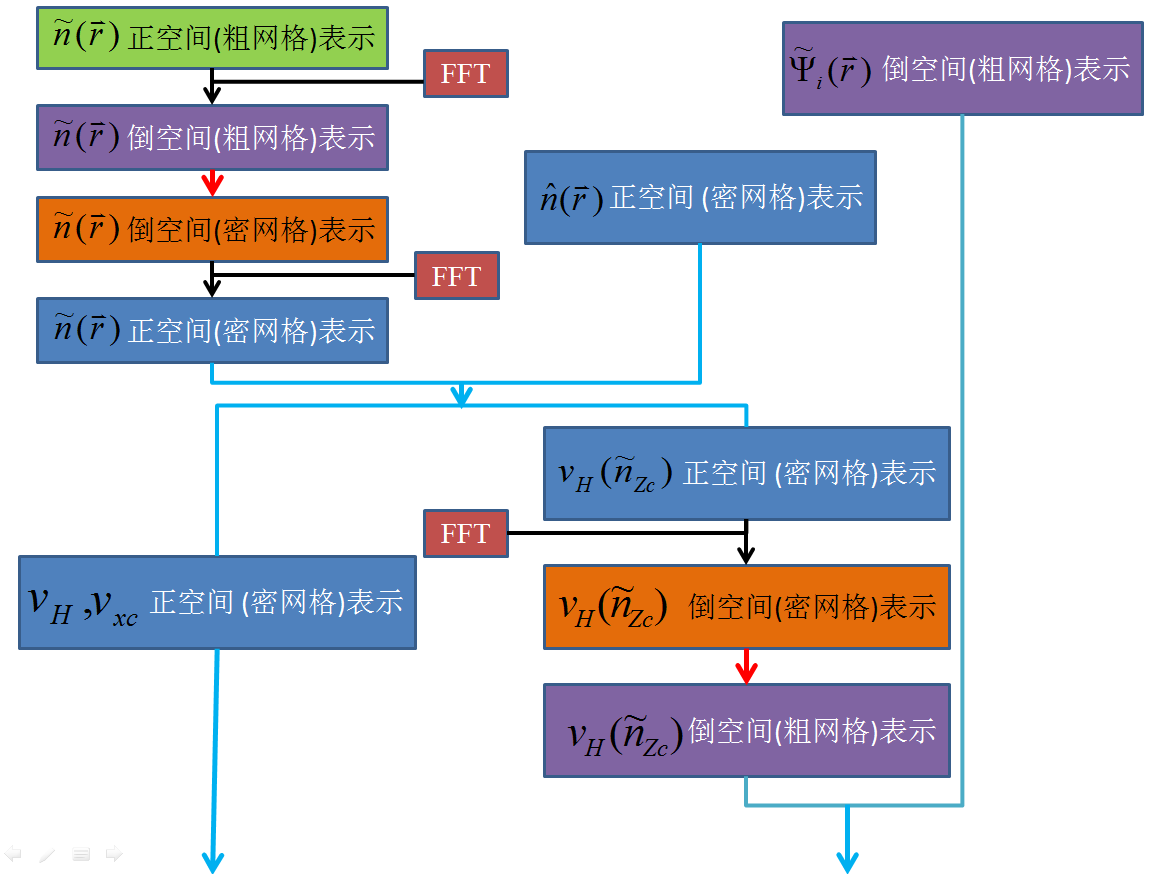
\includegraphics[height=2.7in,width=4.0in,viewport=0 0 1180 875,clip]{Figures/dual_grid.png}
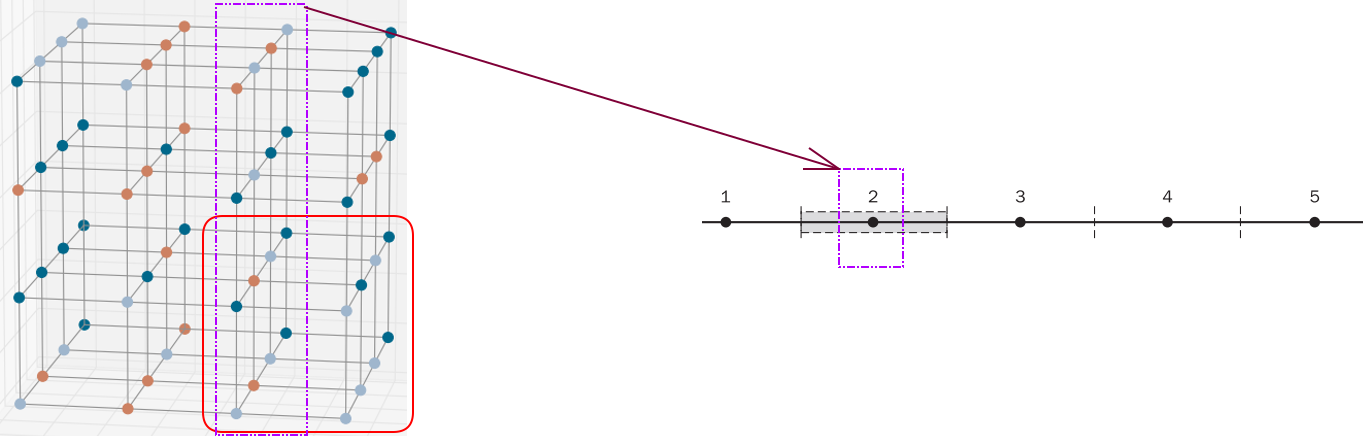
\includegraphics[height=1.0in,width=4.0in,viewport=0 0 1500 450,clip]{Figures/VASP_FFT-MPI_Reciprocal.png}
\vskip 0.5pt
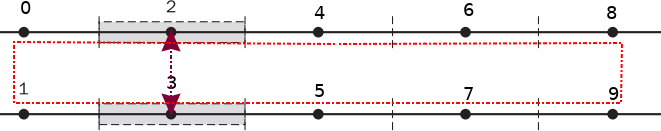
\includegraphics[height=0.7in,width=4.0in,viewport=0 0 730 150,clip]{Figures/VASP_FFT-MPI_Real.png}
\caption{\tiny \textrm{VASP:~ Reciprocal-Real space layout for grids in MPI.}}%(与文献\cite{EPJB33-47_2003}图1对比)
\label{MPI-FFT}
\end{figure} 
	\end{itemize}
}

\frame
{
	\frametitle{\textrm{VASP}的通信开销}
	在高性能的计算队列中,\textrm{VASP}的并行上限可以突破256核,但当并行核数超过百核数量级,并行效率下降非常明显
\begin{figure}[h!]
	\vspace{-0.15in}
\centering
%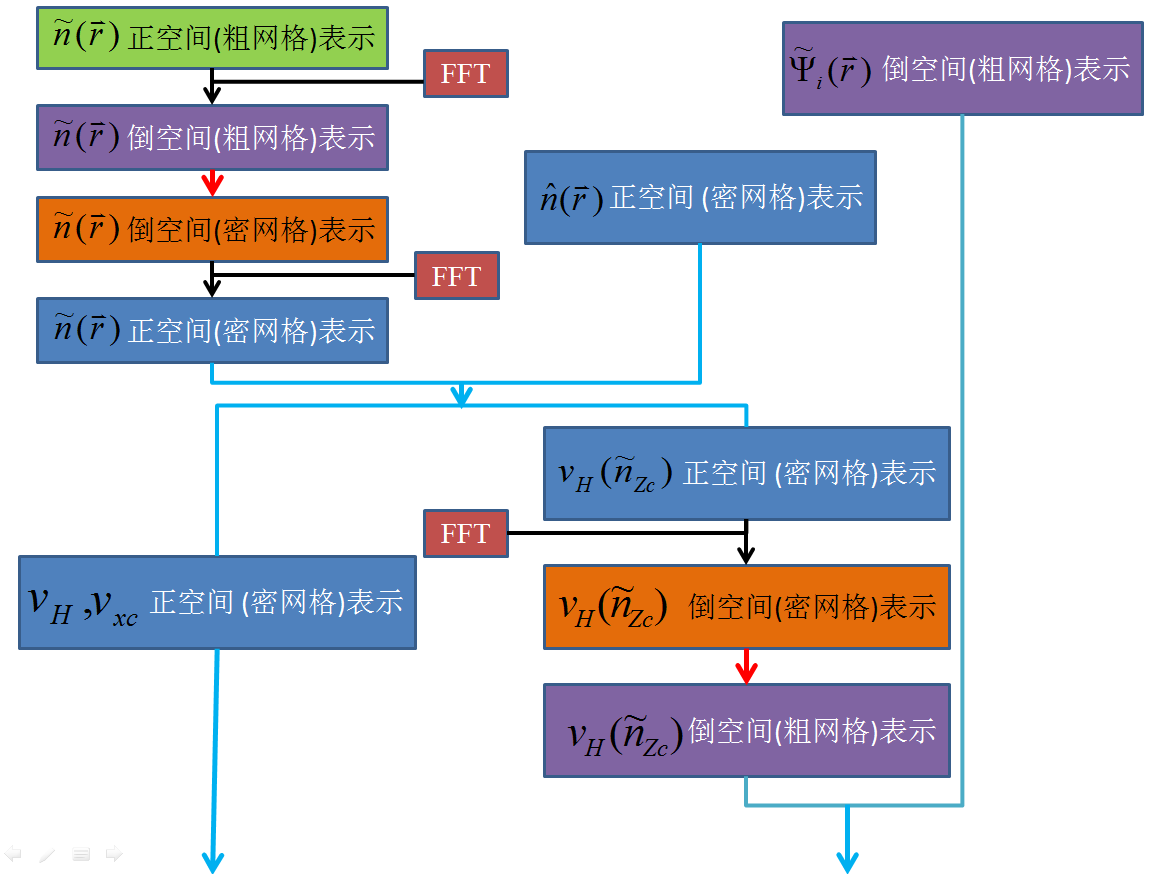
\includegraphics[height=2.7in,width=4.0in,viewport=0 0 1180 875,clip]{Figures/dual_grid.png}
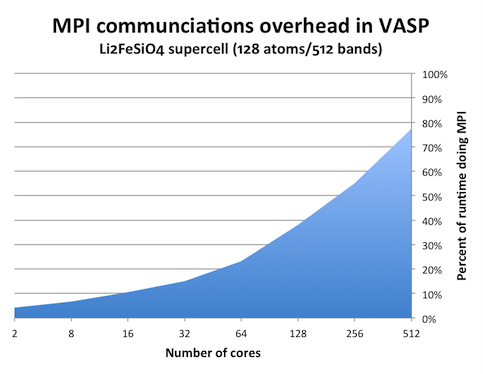
\includegraphics[height=1.55in,width=1.95in,viewport=0 0 240 200,clip]{Figures/VASP-mpi-Li128.png}
\caption{\tiny \textrm{Time spent in MPI calls with increasing the number of ranks in a VASP calculation.}}%(与文献\cite{EPJB33-47_2003}图1对比)
\label{VASP_communication}
\end{figure} 

如能对并行系统与\textrm{VASP}结合作深度改造(如国家超算天津中心方案),\textrm{VASP}的并行扩展可以到$10^4$核级别,但这一改造需要对底层代码和计算框架作较大规模改动
}

\frame
{
	\frametitle{\textrm{VASP}的\textrm{GPU}加速}
\textrm{NVIDIA}多年来致力于\textrm{VASP}的\textrm{GPU}加速,取得了一定的成效
\begin{figure}[h!]
	\vspace{-0.15in}
\centering
%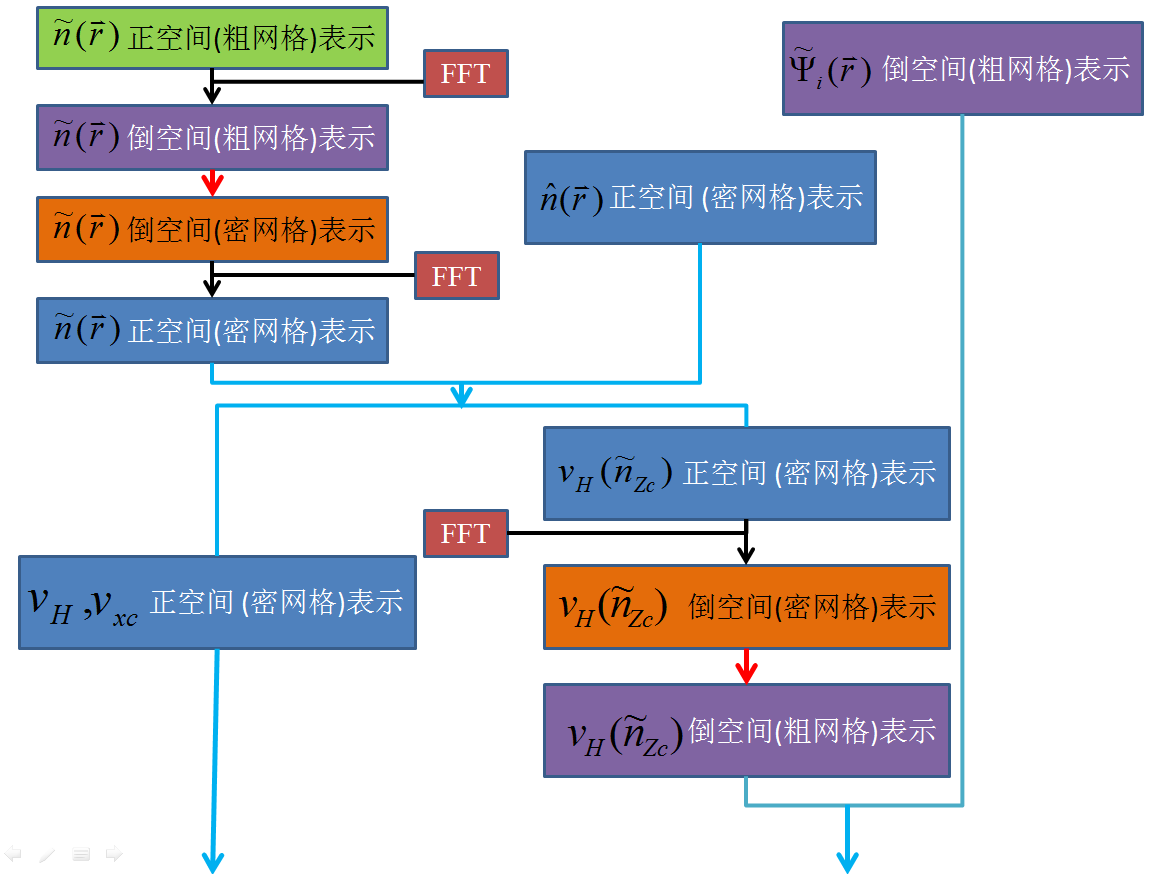
\includegraphics[height=2.7in,width=4.0in,viewport=0 0 1180 875,clip]{Figures/dual_grid.png}
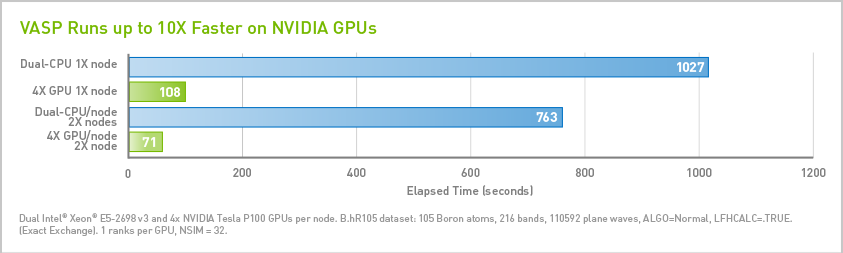
\includegraphics[height=1.2in,width=4.05in,viewport=0 0 850 260,clip]{Figures/VASP-GPU-CPU.png}
\caption{\tiny \textrm{Compare of VASP calculation with GPU and CPU.}}%(与文献\cite{EPJB33-47_2003}图1对比)
\label{VASP_GPU}
\end{figure} 
\begin{itemize}
	\item 通用配置下,\textrm{GPU}对\textrm{VASP}计算有加速效果,一般可提升4$\sim$6倍
	\item 矩阵对角化的并行算法限制了\textrm{GPU}在第一原理计算中的应用
	\item \textrm{GPU}加速的模式主要适合于分子动力学计算
\end{itemize}
}

%\frame[allowframebreaks]
\section{\textrm{VASP}中的电荷密度混合与矩阵迭代对角化}
\frame
{
	\frametitle{\textrm{VASP}的优化与迭代收敛}
	\textrm{VASP}计算中,资源消耗的主要部分是求解\textrm{Kohn-Sham}方程,即偏微分方程\textrm{(Partial Differential Equations,~PDE)}的自洽迭代, 迭代过程主要包括
	\begin{itemize}
		\item 矩阵的迭代对角化
		\item 电荷密度的自洽迭代
	\end{itemize}

	\vskip 10pt
	\textrm{VASP}的计算高效得益于求解过程中中应用了多种经典优化算法,保证了迭代计算的快速收敛\upcite{CMS6-15_1996,PRB54-11169_1996}
	\begin{itemize} 
		\item 拟牛顿法\textrm{(Quasi-Newton method)}
		\item 共轭梯度法\textrm{(Conjugate Gradients method, CG)}
		\item 残差最小化\textrm{(RMM-DIIS)}方法
	\end{itemize}
}

\frame[allowframebreaks]
{
	\frametitle{电荷密度混合收敛算法}
	根据\textrm{DFT},搜索基态电荷密度的过程就是能量泛函优化的过程,可以通过此前讨论的迭代算法实现:\\
%由初猜电荷密度出发,
	\begin{displaymath}
		R[\rho_{\mathrm{in}}]=\rho_{\mathrm{out}}[\rho_{\mathrm{in}}]-\rho_{\mathrm{in}}
	\end{displaymath}
	自洽迭代收敛时,残矢模量$\langle R[\rho_{\mathrm{in}}]|R[\rho_{\mathrm{in}}]\rangle~\rightarrow~0$

	\begin{itemize}
		\item 线性混合:\\
			如果电荷密度自洽迭代的每一步只保留当前步的电荷密度信息,就是线性电荷密度的线性混合
			\begin{displaymath}
				\rho_{\mathrm{in}}^{m+1}=\rho_{\mathrm{in}}^{m}+\gamma R[\rho_{\mathrm{in}}^m]
			\end{displaymath}
	显然,这种线性混合收敛比较慢,应用\textrm{Jacobian}矩阵相关的知识,通过选择\textrm{Preconditioning~}函数,加速自洽迭代的收敛
	\begin{displaymath}
		\rho_{\mathrm{in}}^{m+1}=\rho_{\mathrm{in}}^{m}+\mathbf{G}^1R[\rho_{\mathrm{in}}^m]
	\end{displaymath}
		\item \textrm{Kerker~}混合:\\%~
			以平面波为基,选择的\textrm{Preconditioning~}函数为
			\begin{displaymath}
				G_q^1=A\dfrac{q^2}{q^2+q_0^2}\quad\mbox{一般取$A=0.8$,$q_0$则可根据体系优化}
			\end{displaymath}
		\item \textrm{Pulay}混合:\\
			优化过程中,保留此前若干步的输入电荷密度和残矢,用于迭代的优化电荷密度由此前的电荷密度线性组合得到
			\begin{displaymath}
				\rho_{\mathrm{in}}^{\mathrm{opt}}=\sum_i\alpha_i\rho_{\mathrm{in}}^i
			\end{displaymath}
			\textcolor{magenta}{假设残矢与密度有相同的线性化形式}
			\begin{displaymath}
				R[\rho_{\mathrm{in}}^{\mathrm{opt}}]=R\bigg[\sum_i\alpha_i\rho_{\mathrm{in}}^i\bigg]=\sum_i\alpha_iR[\rho_{\mathrm{in}}^i]
			\end{displaymath}
			在归一化约束条件$\sum\limits {i}\alpha_i=1$下,通过最小化残矢模量$\langle R\big[\rho_{\mathrm{in}}^{\mathrm{opt}}\big]|R\big[\rho_{\mathrm{in}}^{\mathrm{opt}}\big]\rangle$,得到优化电荷密度,可以得到优化系数$\alpha_i$
	\begin{displaymath}
		a_i=\dfrac{\sum\limits_{j}A_{j,i}^{-1}}{\sum\limits_{j,k}A_{j,k}^{-1}}\qquad A_{j,k}=\langle R[\rho_{\mathrm{in}}^{j}]|R[\rho_{\mathrm{in}}^{k}]\rangle 
	\end{displaymath}
\item \textrm{Brondey}混合:\\
	这是所有自洽求解\textrm{Kohn-Sham}方程方法中最复杂的,属于准-\textrm{Newton}类方法。在迭代过程中,用近似方法不断对\textrm{Jacobian~}矩阵(或逆矩阵)逼近\\
	每次自洽迭代中并不需要保存全部$N\times N$的\textrm{Jacobian}矩阵,只需要存储$N$-维矢量\\
	\textcolor{purple}{残矢可以线性化地表示为}
	\begin{displaymath}
		R[\rho]=R[\rho_{\mathrm{in}}^m]-\mathrm{J}^m(\rho-\rho_{\mathrm{in}}^m)
	\end{displaymath}
	这里$\mathbf{J}^m$是对\textrm{Jacobian~}矩阵的近似($(\mathbf{J}^m)^{-1}$是\textrm{Jacobian}矩阵的逆阵,习惯上取$\mathbf{G}^m=(\mathbf{J}^m)^{-1}$),由此可有迭代电荷密度
	\begin{displaymath}
		\rho_{\mathrm{in}}^{m+1}=\rho_{\mathrm{in}}^m+(\mathbf{J}^m)^{-1}R[\rho_{\mathrm{in}}^m]
	\end{displaymath}
	此类方法因为迭代中$\mathbf{J}^m$的变化形式不同,可以选择多种方案\\
	定义误差函数
	\begin{displaymath}
		E=w_0||\mathbf{G}^{m+1}-\mathbf{G}^m||^2+\sum_{i=1}^mw_i||\Delta\rho^i+\mathbf{G}^{m+1}\Delta R^i||^2
	\end{displaymath}
	这里$||A||^2=\langle A|A\rangle$,$w_i$是权重因子,并且有
	\begin{displaymath}
		\begin{aligned}
			\Delta\rho^i=&\rho_{\mathrm{in}}^{i+1}-\rho_{\mathrm{in}}^{i}\\
			\Delta R[\rho^i]=&R[\rho_{\mathrm{in}}^{i+1}]-R[\rho_{\mathrm{in}}^{i}]
		\end{aligned}
	\end{displaymath}
	\begin{itemize}
		\item 误差函数的第一项要求\textrm{Jacobian}矩阵的逆阵在迭代中变化不大,并有$w_0\rightarrow0$
		\item 误差函数的第二项要求模$||\Delta\rho^i+\mathbf{G}^{m+1}\Delta R^i||$足够小
	\end{itemize}
	用最小二乘法确定最小化误差,可以确定$\mathbf{G}^m$
	\begin{displaymath}
		\mathbf{G}^{m+1}=\mathrm{G}^1-\sum_{k=1}^m|\mathbf{Z}_k^m\rangle\langle\Delta R^k|
	\end{displaymath}
	其中
	\begin{displaymath}
		\begin{aligned}
			|\mathbf{Z}_k^m\rangle=&\sum_{n=1}^m\beta_{kn}w_kw_n|u^n\rangle+\sum_{n=1}^{m-1}\bar{\beta}_{kn}|\mathbf{Z}_n^{m-1}\rangle\\
			|u^n\rangle=&\mathbf{G}^1|\Delta R^n\rangle+|\Delta \rho^n\rangle
		\end{aligned}
	\end{displaymath}
	而$\beta_{kn}$和$\bar\beta_{kn}$由下式给出
	\begin{displaymath}
		\begin{aligned}
			\beta_{kn}=&\big(w_0^2+\bar A\big)_{kn}^{-1},\qquad \bar A_{kn}=w_kw_n\langle\Delta R^n|\Delta R^k\rangle\\
			\bar\beta_{kn}=&\delta_{kn}-\sum_{j=1}^mw_kw_j\beta_{kj}\langle\Delta R^n|\Delta R^j\rangle
		\end{aligned}
	\end{displaymath}
		{\fontsize{7.2pt}{4.2pt}\selectfont{
	不难看出\\$w_0\rightarrow 0$并且$w_0\ll w_n$,该方法就得到\textrm{Pulay}方法\\
	而一旦$w_0\rightarrow 0$时,$w_n$的选择,完全不会影响$\mathbf{G}^{m+1}$,因此取$w_n=1$可有
	\begin{displaymath}
		\mathbf{G}^m=\mathbf{G}^1-\sum_{k,n=1}^{m-1}\beta_{kn}|u^n\rangle\langle\Delta R^k|
	\end{displaymath}
而如果令$w_i=0$并要求$w_0\ll w_m$,有
\begin{displaymath}
	\begin{aligned}
		|\mathbf{Z}_k^m\rangle=&|\mathbf{Z}_k^{m-1}\rangle\qquad k<m\\
		|\mathbf{Z}_m^m\rangle=&\dfrac1{||\Delta R^m||^2}\bigg(|u^m\rangle-\sum_{k=1}^{m-1}\langle\Delta R^k|\Delta R^m\rangle|\mathbf{Z}_k^{m-1}\rangle\bigg)
	\end{aligned}
\end{displaymath}
}}
	\end{itemize}
}

\frame
{
	\frametitle{矩阵的迭代对角化}
	\begin{itemize}
		\item 矩阵的直接对角化计算复杂复 $O(N^3)$
		\item 矩阵的迭代对角化计算复杂度 $O(N_0^2\times N\ln N)\quad N_0\ll N$
	\end{itemize}
	\textcolor{blue}{迭代求本征值的思想是\textrm{Jacobian~}于\textrm{1846~}年提出的}\upcite{Crelle30-51_1846}\\
	其基本思想是
	\begin{displaymath}
		(H-\varepsilon^n)|\psi^n\rangle=|R[\psi^n]\rangle
	\end{displaymath}
	这里$n$是迭代步数,$|\psi^n\rangle$和$\varepsilon^n$分别是本征态和本征值,$|R[\psi^n]\rangle$是残差矢量
	\vskip 10pt
	{\fontsize{7.2pt}{1.2pt}\selectfont{
	在电子态计算过程中,选择适当的基函数,可以使\textrm{Schr\"odinger~}方程的矩阵接近对角阵\\因此可有
	\begin{displaymath}
		\begin{aligned}
			|\psi^{n+1}\rangle=&\mathbf{D}^{-1}(\mathbf{H}-\varepsilon)|\psi^n\rangle+|\psi^n\rangle=\delta|\psi^{n+1}\rangle+|\psi^n\rangle\\
		\mathbf{D}\delta\psi^{n+1}=&R[\psi^n]
		\end{aligned}
	\end{displaymath}
	这里$\mathbf{D}$是非奇异矩阵,与$\mathbf{H}$矩阵有关,也叫''预处理矩阵'',可根据需要选取多种形式
	\begin{itemize}
		\item 要求$\mathbf{D}$比原始的$\mathbf{H}-\varepsilon$更易求逆阵
		\item 要求$\mathbf{D}$使得修正项$\delta\psi^{n+1}$能够使$\psi^n$尽可能接近正确的本征矢
	\end{itemize}
}}
}

\frame
{
	\frametitle{矩阵的迭代对角化}
	``预处理矩阵''%$\mathbf{K}$
	的作用,是使\textcolor{red}{函数(泛函)对变量的依赖趋于“同质”(\textrm{isotropic})},即函数曲线与不同变量的依赖关系趋同

	具体到电子结构求解:~
	\begin{itemize}
		\item \textcolor{blue}{平面波基}\\
			基函数$\mathrm{e}^{\mathrm{i}\vec G_m\cdot\vec r}$对波函数$\psi_{\vec k_i+\vec G}^n(\vec r)$的贡献为$c_{i,m}^n(\vec k)$\\
		{\fontsize{7.2pt}{4.2pt}\selectfont{
		在能量泛函表达式中,高频(大的$\vec G_m$)部分比低频(小的$\vec G_m$)贡献大得多}}\\
			\textrm{preconditioning}\textcolor{blue}{要使不同频率对能量泛函贡献趋同}:\\
			\textcolor{red}{不同本征矢的修正项趋同,而与相应的能量本征值无关。}取
	\begin{displaymath}
		K(x)=\dfrac{27+18x+12x^2+8x^3}{27+18x+12x^2+8x^3+16x^4}
	\end{displaymath}
	此处定义
	\begin{displaymath}
		x_i^n(\vec G_m)=\dfrac12\dfrac{|\vec k+\vec G_m|^2}{E^{\mathrm{kin}}(\mathbf{R}^n)}
	\end{displaymath}
	\textcolor{purple}{$x_i^n(\vec G_m)$表示对$n$次迭代后本征态$i$中平面波组分$|\vec k_i+\vec G_m|$动能贡献的调整比例}
	\end{itemize}
}

\frame
{
	\frametitle{矩阵迭代对角化}
	稀疏矩阵求解的\textrm{Lanczos}优化过程\upcite{Elect_Stru,Comp_Phys},只变动一个分量$\mathbf{c}_I$的前提下
	\begin{displaymath}
		\dfrac{\partial\rho}{\partial\mathbf{c}_I}\bigg|_{\mathbf{c}_I+\delta_I}=0
	\end{displaymath}
	是可以精确求解的,其解为
	\begin{displaymath}
		\delta_I=(\rho(\mathbf{c}_0)-\mathbf{H}_{II})^{-1}\mathbf{q}_I\qquad\mbox{这里}\mathbf{q}=(\mathbf{H}-\rho\mathbf{I})\mathbf{c}_0
	\end{displaymath}
	不难看出,矢量$\mathbf{q}$就对应\textrm{Jacobi}迭代中用于判断收敛的残差矢量

更一般地,求解方程
	\begin{displaymath}
		\dfrac{\partial\rho}{\partial\mathbf{c}}\bigg|_{\mathbf{c}+\mathbf{\delta}}=0
	\end{displaymath}
	将方程展开到二阶近似,不难有
	\begin{displaymath}
		(\rho-\mathbf{H}_{II})\delta_I\approx \mathbf{q}_I+\sum_{J\neq I}\delta_J+(\rho-\lambda)\mathbf{c}_I
	\end{displaymath}
	实际计算中选则$\delta_I=(\rho(\mathbf{c}_0)-\mathbf{H}_{II})^{-1}\mathbf{q}_I$并不是方程的解的好的近似,\textcolor{purple}{好处是计算比较简单}
}

\frame
{
	\frametitle{\textrm{Block-Davison algorithm}}
	\textrm{Davidson}方法是求解大型稀疏矩阵的少量本征值问题提出来的,结合了\textrm{Lanczos}优化和\textrm{Jacobi}迭代的优点,简言之就是改进初猜,不用$\mathbf{H}\mathbf{c}_0$,而改用计算简单的$\delta_I=(\rho(\mathbf{c}_0)-\mathbf{H}_{II})^{-1}\mathbf{q}_I$形式
	\vskip 10pt
	应用\textrm{Davison}方法可以快速地依次求解稀疏矩阵的少量本征值和本征矢,将该方法推广为同时求解若干个本征态,即块-\textrm{Davidson}方法
	{\fontsize{6.2pt}{1.2pt}\selectfont{
		\begin{itemize}
			\item 选取合适数目正交归一的向量$\mathbf{c}_1,\mathbf{c}_2,\cdots, \mathbf{c}_n$作为初猜子空间的基组, 计算并储存向量$\mathbf{H}\mathbf{c}_i$和矩阵元$\mathbf{H}=\langle\mathbf{c}_i|\mathbf{H}|\mathbf{c}_j\rangle$ 
			\item 对角化矩阵,得到本征值$\lambda^{n}$和本征矢$\mathbf{a}^{n}$
			\item 构造残量矢量$\mathbf{q}_M=(\mathbf{H}-\lambda^{(M)}\mathbf{I})\mathbf{a}^{(M)}~\mbox{其中}\mathbf{a}^{(M)}=\sum\limits_{i=1}^M a_i^{(M)}\mathbf{a}_i$
			\item 根据模长$||\mathbf{q}_M||$判断迭代收敛情况
			\item 构造$\delta_{I,M+1}=(\lambda^{(M)}-\mathbf{H}_{II})^{-1}\mathbf{q}_{I,M}$,与此前的基组正交归一化,得到$\mathbf{c}_{M+1}$
			\item 计算矩阵元$\mathbf{H}_{i,M+1}\quad i=1,2,\cdots, M+1$
			\item 对角化矩阵得到新的本征值和本征矢量,继续迭代
		\end{itemize}
	}}
}

\frame
{
	\frametitle{\textrm{RMM-DIIS}}
	{\fontsize{7.2pt}{1.2pt}\selectfont{前述矩阵迭代对角化方法的优化策略都是
	\begin{itemize}
		\item 通过迭代优化得到最小本征值(极值)
		\item 利用本征态正交,依次获得其他各本征态和本征值
	\end{itemize}}}
	{\fontsize{7.2pt}{1.2pt}\selectfont{\textrm{RMM-DIIS~(Residual Minimization Method by Direct Inversion in the Iterative Subspace)}\footnote{\fontsize{5.2pt}{1.2pt}\selectfont{\textrm{RMM-DIIS}的得名源自该方法的提出者\textrm{Pulay}:~该方法的基本思想是在历次迭代产生的矢量构成的完整\textrm{Krylov}子空间内,完成对残矢的最小化}}方法则可以不用引入正交条件而得到多个本征值,\textcolor{purple}{因为该方法最小化的不是本征值而是残矢}}}\\
	{\fontsize{5.2pt}{1.2pt}\selectfont{
		其基本思想概要:~在$n$维\textrm{Krylov}子空间内,生成矢量
		\begin{displaymath}
			\psi^{n+1}=c_0\psi^0+\sum_{j=1}^{n+1}c_j\delta\psi^{j}
		\end{displaymath}
		通过改变选取一套合适的系数$c_j$来完成$\psi^{n+1}$的残矢$R^{n=1}$的最小化。\textcolor{blue}{等价于$c_j$由$\{\psi^0,\psi^1,\cdots,\psi^n\}$构成的\textrm{Krylov}子空间内求\textrm{Hermitian}本征值问题}
		\begin{displaymath}
			\sum_{j=1}^n\langle R^i|R^j\rangle c_j=\varepsilon\sum_{j=1}^n\psi^i|\mathbf{S}|\psi^j\rangle c_j
		\end{displaymath}
		每迭代一次,子空间引入一个新波函数$\psi$和一个新残矢$R(\psi)$
		\begin{itemize}
			\item \textrm{RMM-DIIS}的计算量瓶颈将是后续的逐个矩阵-向量乘操作$\textrm{H}\psi$
%				\\因此要避免直接用\textrm{RMM-DIIS}直接处理大规模本征态~(但可以是大体系中的少量本征态)
			\item 只要内存许可,\textrm{RMM-DIIS}构造的完整的子空间内,构成子空间的矢量本征值都可以求解出来
			\item 因为\textrm{RMM}方法对初猜的矢量敏感(矢量收敛的位置到离初猜较近)
		\end{itemize}
%		\textrm{RMM-DIIS}最大的优点是一次可以得到多个本征态和本征值,而且不需要正交化
	}}
}

%\frame
%{
%	\frametitle{矩阵的迭代对角化}
%	\begin{itemize}
%		\item \textcolor{blue}{实空间基}\\
%		与平面波基类似,可以定义
%	\begin{displaymath}
%		x_i^n(\vec r)=A\dfrac12\dfrac{\lambda_i^m-V(\vec r)}{E^{\mathrm{kin}}(\mathbf{R}^n)}
%	\end{displaymath}
%		\textcolor{purple}{$x_i^n(\vec r)$表示对$n$次迭代后本征态$i$中局部动能$|\lambda_i-V(\vec r)|$对总动能贡献的调整比例}
%	\end{itemize}
%	完成\textrm{preconditioning}得到矩阵$\mathbf{K}(x_i^n)$后,由
%	\begin{displaymath}
%		\psi^{n+1}\equiv\mathbf{K}\mathbf{R}^n
%	\end{displaymath}
%	可根据残矢量$\mathbf{R}^n$选择方式的不同,将\textcolor{blue}{\textrm{SD}、\textrm{CG}}、\textcolor{blue}{\textrm{RMM-DIIS}}等多种算法应用于矩阵迭代对角化计算
%}
%
\section{\rm{VASP}计算的原子数据重建}
\frame
{
	\frametitle{\textrm{VASP}计算的原子数据基础}
	\textrm{POTCAR}提供了\textrm{VASP}计算所需的原子数据,也是实现\textrm{PAW}方法的主要基础
	\begin{itemize}
		\item \textrm{POTCAR}是\textrm{VASP}实现材料精确计算的重要保证\\
			同样都应用\textrm{PAW}方法,\textcolor{blue}{公认\textrm{VASP}较\textrm{QE}、\textrm{ABINIT}等软件的计算精度要高}
		\item \textrm{POTCAR}数据生成依赖较多的可调参数\\
			包括能量参数$\varepsilon_l$、多种截断半径$r_c$、$r_{\mathrm{vloc}}$、$r_{\mathrm{shape}}$、$r_{\mathrm{core}}$
		\item \textcolor{red}{\textrm{POTCAR}数据生成代码是\textrm{VASP}中唯一没有公开的}
		\item 用\textrm{VASP}模拟极端条件下材料物性的能力,受到\textrm{POTCAR}数据的制约
	\end{itemize}
	%文献\cite{PRB59-1758_1999}介绍了\textrm{POTCAR}的主要实现思想

当前研究主要尝试基于开源的\textrm{PAW}赝势生成软件(\textrm{atomPAW}),开发能生成\textrm{POTCAR}原子数据的功能
}

\frame
{
	\frametitle{\textrm{PAW}原子数据集:~\textrm{wave~function}}
	平滑赝原子分波函数
	\begin{displaymath}
		\tilde\phi_{i=Lk}(\vec r)=Y_L(\widehat{\vec r-\vec R})\tilde\phi_{lk}(|\vec r-\vec R|)
	\end{displaymath}
	根据\textrm{RRKJ}赝势构造的思想,赝分波函数由球\textrm{Bessel}函数线性组合%\upcite{JPCM6-8245_1994}
	\begin{displaymath}
		\tilde\phi_{lk}(r)=\left\{
		\begin{aligned}
			&\sum_{i=1}^2\alpha_ij_l(q_ir)\quad &r<r_c^l\\
			&\phi_{lk}(r)\quad&r>r_c^l
		\end{aligned}
		\right.
	\end{displaymath}
	调节系数$\alpha_i$和$q_i$赝分波函数$\phi_{lk}(r)$在截断半径$r_c^l$处两阶连续可微
%	投影子波函数$\tilde p_i$由\textrm{Gram-Schmidt}正交条件$\langle\tilde p_i|\tilde\phi_j\rangle=\delta_{ij}$确定
}

\frame
{
	\frametitle{\textrm{PAW}原子数据集:~\textrm{wave~function}}
\begin{figure}[h!]
\centering
\vskip -0.5in
\includegraphics[width=1.5in,height=2.7in,viewport=0 0 350 550, angle=-90, clip]{Figures/WAE-data.eps}
\vskip -0.2in
\includegraphics[height=2.7in,width=1.5in,viewport=0 0 350 550, angle=-90, clip]{Figures/WPS-data.eps}
\caption{\tiny \textrm{The partial wave function.}}%(与文献\cite{EPJB33-47_2003}图1对比)
\label{Wave_Function}
\end{figure}
}

\frame
{
	\frametitle{\textrm{PAW}原子数据集:~\textrm{core~density}}
	\textcolor{blue}{构造赝芯电荷密度$\tilde n_c$}:~在截断半径$r_{\mathrm{core}}$内的定义为
	$$\sum_{i=1,2}B_i\dfrac{\sin(q_ir)}r\quad r<r_{\mathrm{core}}$$
	调节系数$q_i$和$B_i$使得赝芯电荷密度$\tilde n_c(r)$在截断半径$r_{\mathrm{core}}$处的两阶导数连续
\begin{figure}[h!]
\vskip -0.5in
\centering
\hspace*{-0.1in}
\includegraphics[width=1.5in,height=2.35in,viewport=0 0 350 550, angle=-90, clip]{Figures/CORE-data.eps}
\hspace*{-0.7in}
\includegraphics[height=2.35in,width=1.5in,viewport=0 0 350 550, angle=-90, clip]{Figures/PCORE-data.eps}
\caption{\tiny \textrm{The core density.}}%(与文献\cite{EPJB33-47_2003}图1对比)
\label{core_density_Function}
\end{figure}
}

\frame
{
	\frametitle{\textrm{PAW}原子数据集:~$\mathrm{v}_{e\!f\!f}(r)$与$\tilde{\mathrm{v}}_{e\!f\!f}(r)$}
	\textcolor{blue}{原子局域有效势$\mathrm{v}_{e\!f\!f}^a$}
\begin{figure}[h!]
%\vskip -0.5in
\vskip -0.17in
\centering
%\includegraphics[width=1.6in,height=2.7in,viewport=0 0 300 460, angle=-90, clip]{Figures/POTAE-data.eps}
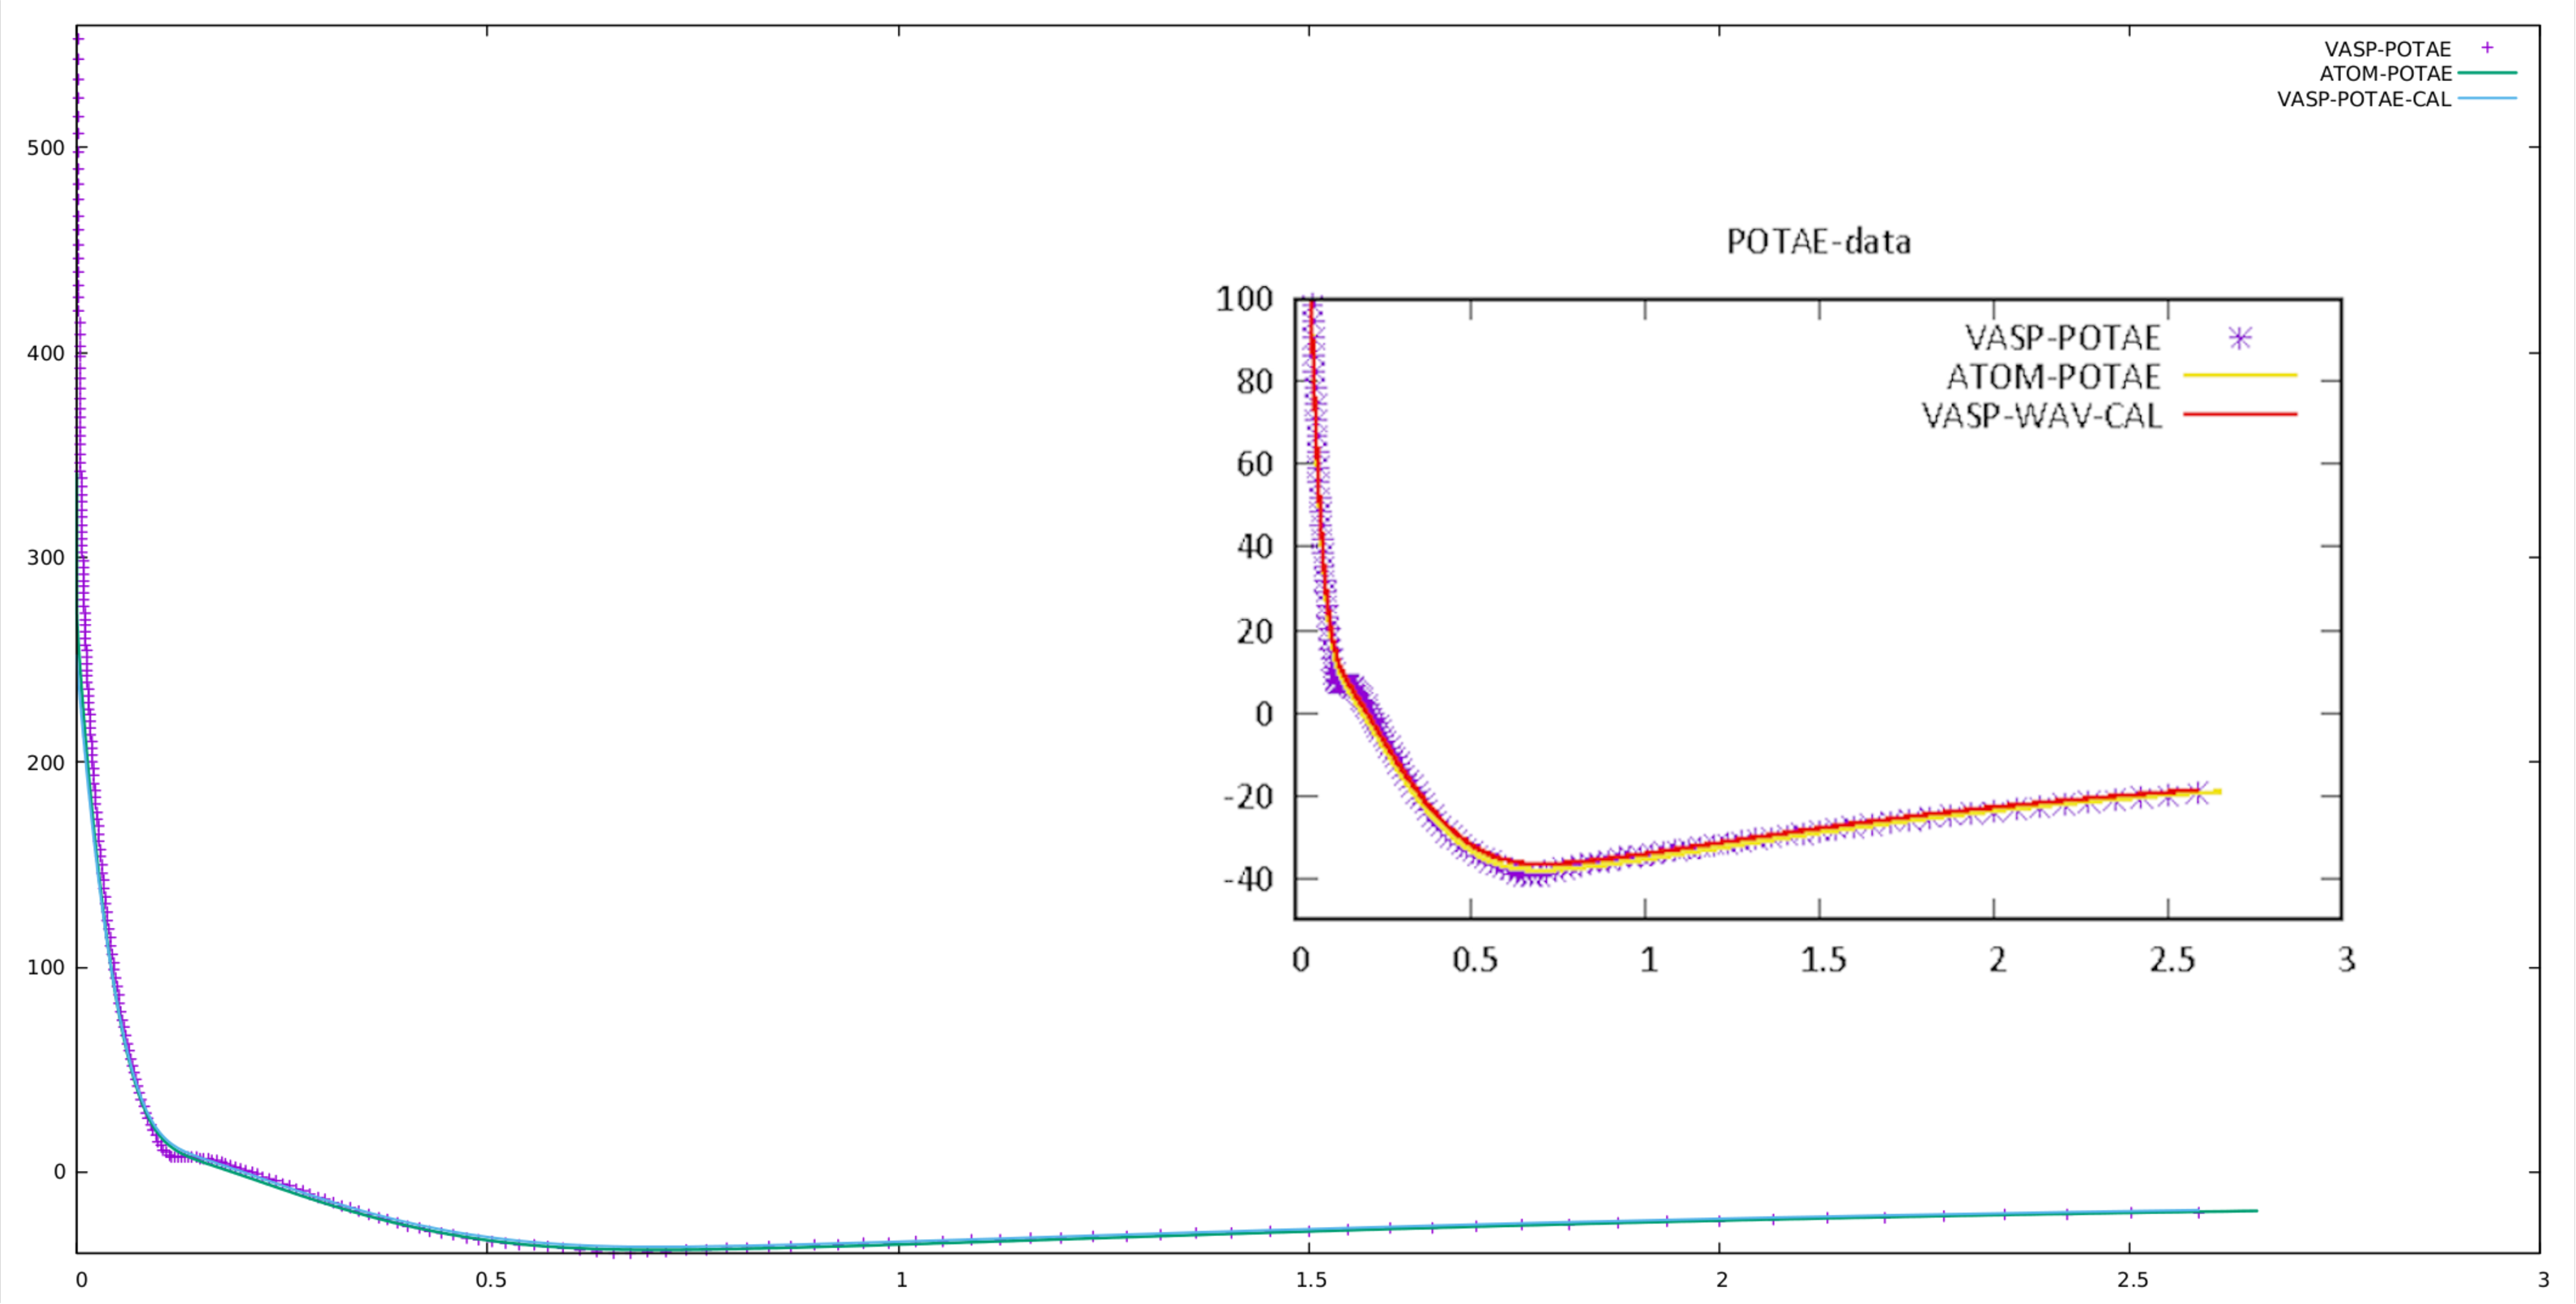
\includegraphics[width=2.5in,height=1.2in,viewport=0 0 1600 800, clip]{Figures/POTAE-full-dat.pdf}
\caption{\tiny \textrm{The local atomic effective-Potential.}}%(与文献\cite{EPJB33-47_2003}图1对比)
\label{local_atomic_PP}
\end{figure}
	\textcolor{blue}{构造原子局域赝势$\tilde v_{e\!f\!f}^a$}%(\textcolor{red}{为防止\textrm{ghost band}})
	:%\\
	(在截断半径$r_{\mathrm{loc}}$内的定义)
	$$\tilde v_{e\!f\!f}^a=A\dfrac{\sin(q_{loc}r)}r\quad r<r_{\mathrm{loc}}$$
	其中$q_{loc}$和$A$要求局域赝势在截断半径$r_{\mathrm{loc}}$处连续到一阶导数
}

\frame
{
	\frametitle{\textrm{PAW}原子数据集:~$\mathrm{v}_H[\tilde n_{Zc}]$}
	局域离子赝势$v_H[\tilde n_{Zc}]$可由原子局域赝势去屏蔽得到
	$$v_H[\tilde n_{Zc}]=\tilde v_{e\!f\!f}^a-v_H[\tilde n_a^1+\hat n_a]-v_{\mathrm{XC}}[\tilde n_a^1+\hat n_a+\tilde n_c]$$
\begin{figure}[h!]
\vskip -0.5in
\centering
\hspace*{-0.1in}
\includegraphics[width=1.5in,height=2.35in,viewport=0 0 350 550, angle=-90, clip]{Figures/POTPS-data.eps}
\hspace*{-0.7in}
\includegraphics[height=2.35in,width=1.5in,viewport=0 0 350 550, angle=-90, clip]{Figures/POTPSC-data.eps}
\caption{\tiny \textrm{The pseudo-potential and local ionic pseudo-potential.}}%(与文献\cite{EPJB33-47_2003}图1对比)
\label{pseudo_potential}
\end{figure}
}

\frame
{
	\frametitle{\textrm{PAW}原子数据集:~$\tilde{n}_{\mathrm G}$}
	局域离子赝势$\tilde{n_{\mathrm G}}$可由原子局域赝密度的\textrm{FFT}得到
\begin{figure}[h!]
\vskip -0.2in
\centering
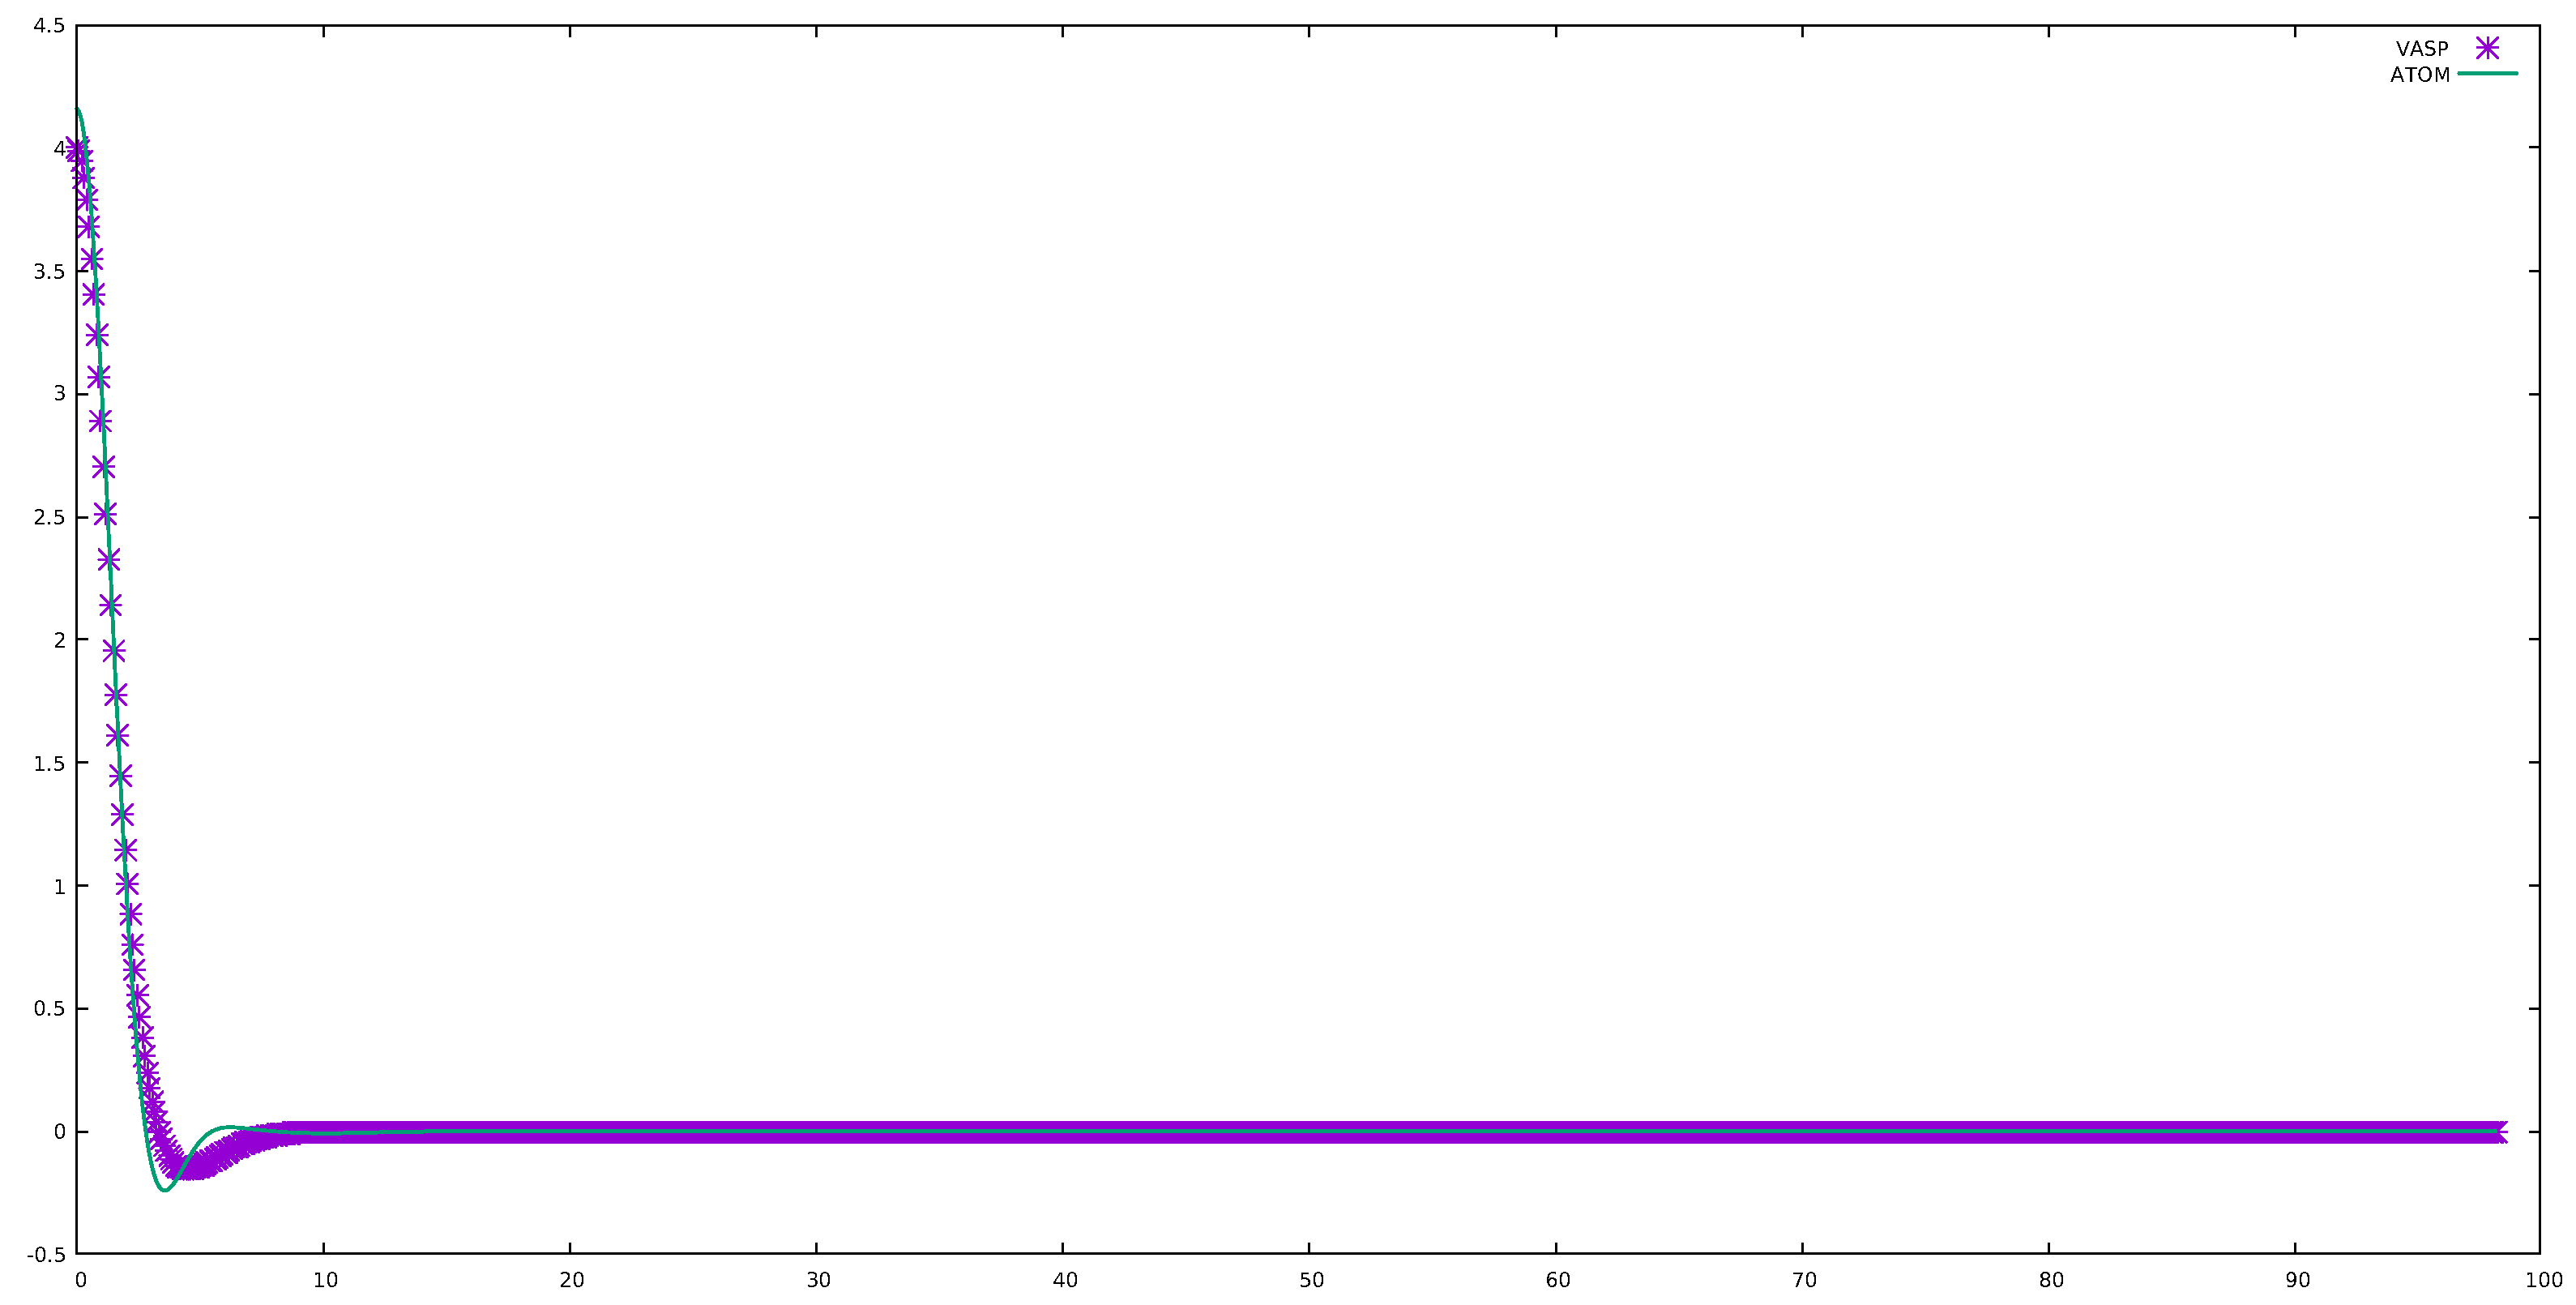
\includegraphics[width=4.0in,height=2.35in,viewport=0 0 1530 850, clip]{Figures/PSRHO_G-dat.pdf}
\caption{\tiny \textrm{The pseudo-density in reciprocal space.}}%(与文献\cite{EPJB33-47_2003}图1对比)
\label{pseudo_density_in_reciprocal-space}
\end{figure}
}

\frame
{
	\frametitle{\textrm{PAW}原子数据集:~$\mathrm{v}_{\mathrm G}[\tilde n_{Zc}]$}
	局域离子赝势在倒空间的表示$v_{\mathrm G}[\tilde n_{Zc}]$可由原子去屏蔽局域赝势的\textrm{FFT}得到
\begin{figure}[h!]
\vskip -0.2in
\centering
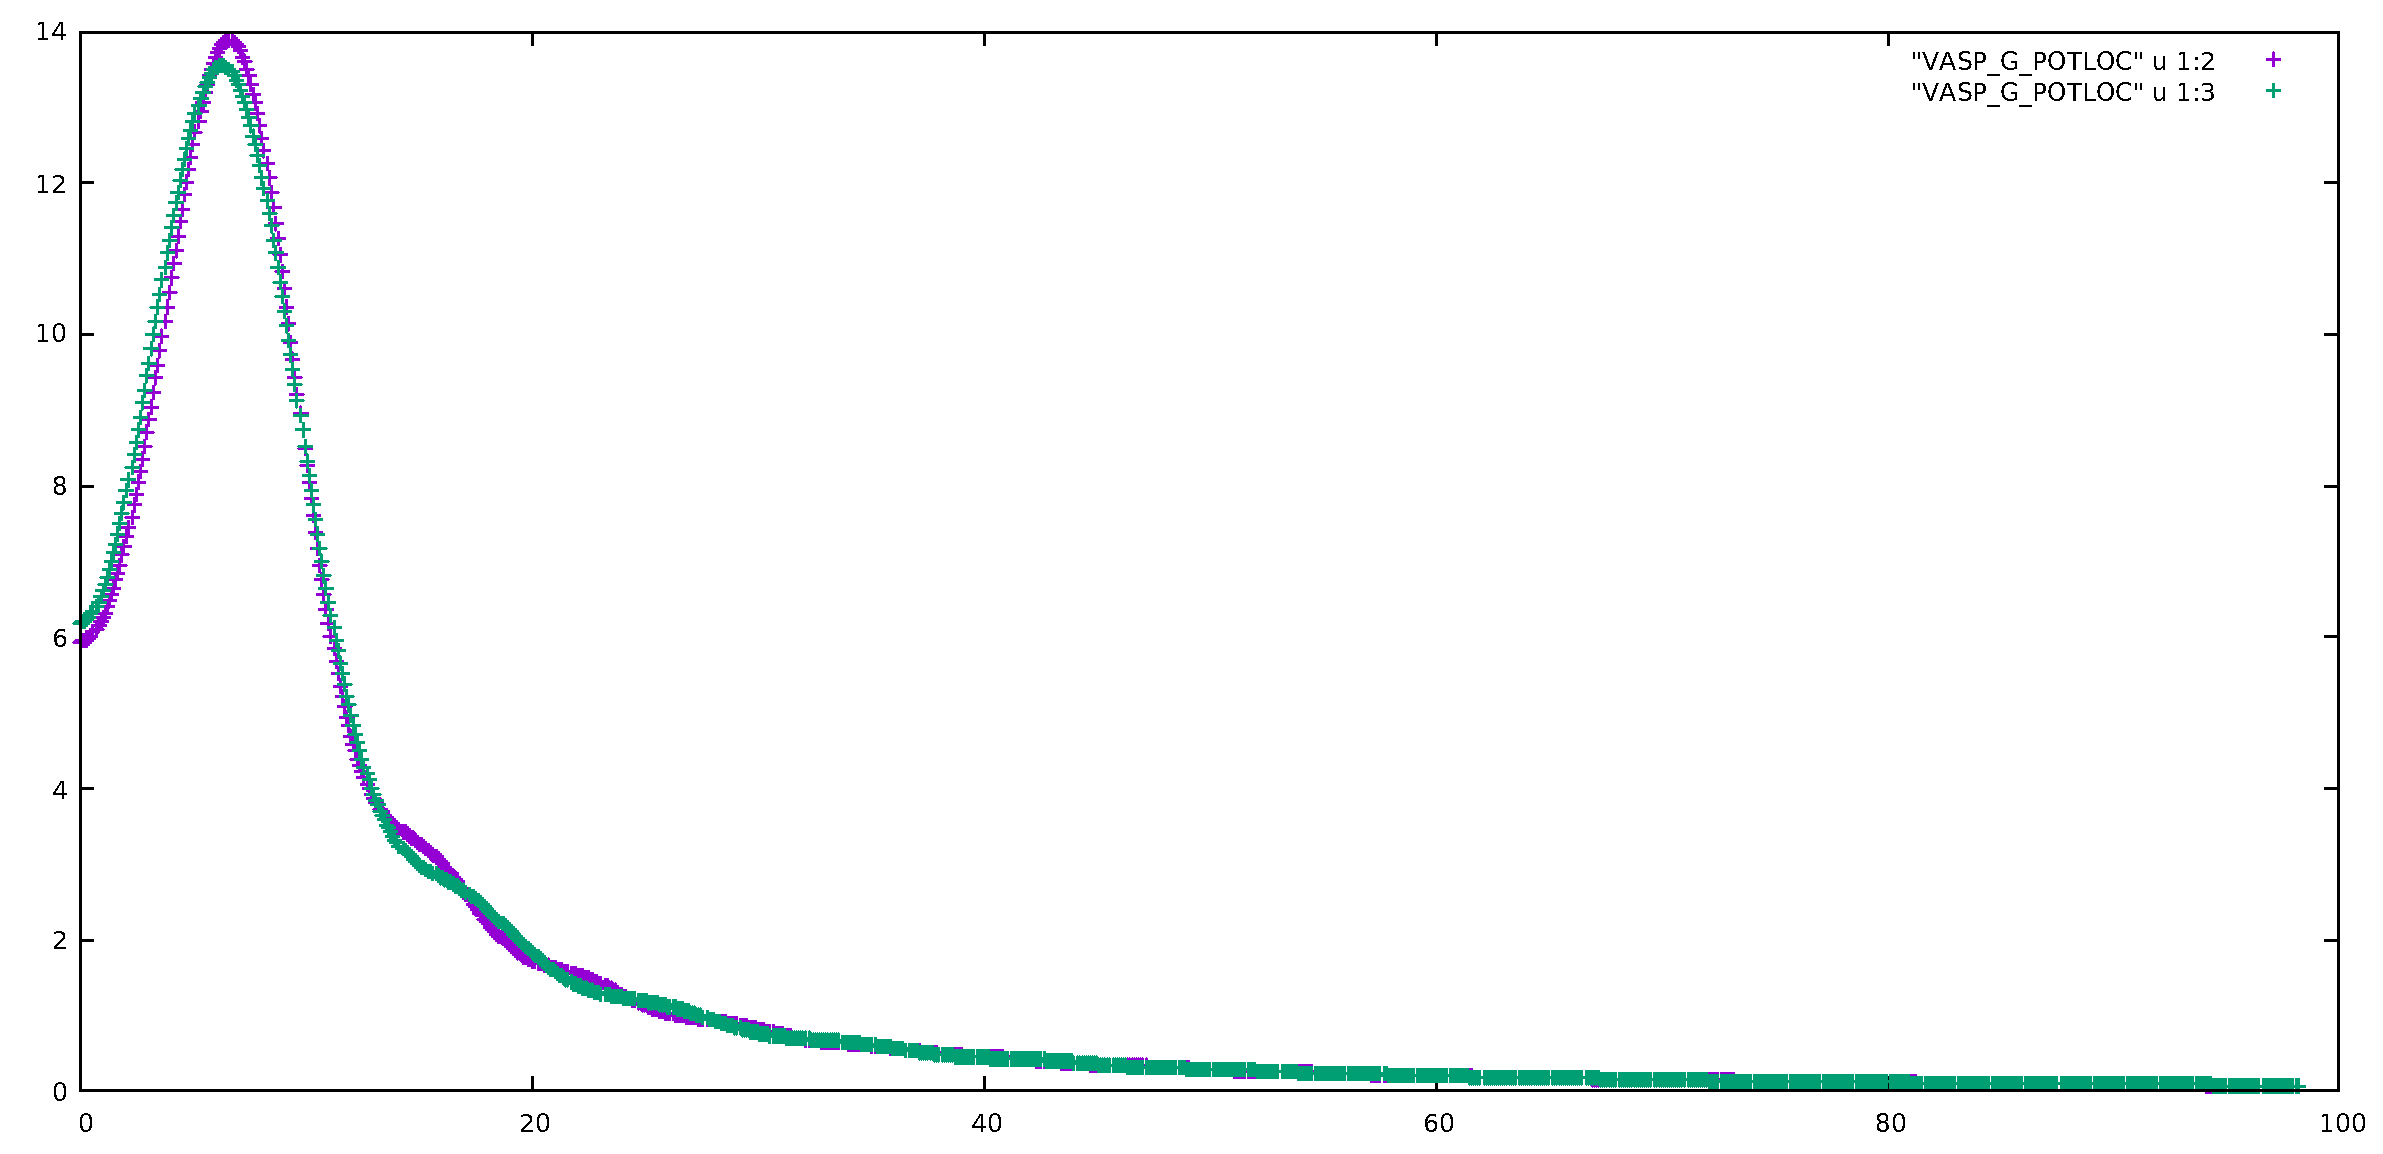
\includegraphics[width=4.0in,height=2.35in,viewport=0 0 1150 650, clip]{Figures/POT_G-dat.pdf}
\caption{\tiny \textrm{The local ionic pseudo-potential in reciprocal space.}}%(与文献\cite{EPJB33-47_2003}图1对比)
\label{pseudo_potential_in_reciprocal-space}
\end{figure}
}

\section{小结}
\frame
{
	\frametitle{小结}
	作为第一性原理计算的商用软件,\textrm{VASP}已成为计算材料学领域应用最广泛的软件之一。全球绝大多数超算中心都安装了\textrm{VASP},据统计,\textrm{VASP}软件的作业机时占用全球总机时的12$\sim$20\%,但由于其%类似于linpack软件,
属于重型浮点计算密集型应用,实际耗电量占比则高达30$\sim$50\%
\vskip 3pt
	{\fontsize{9.0pt}{7.2pt}\selectfont{
	\begin{itemize}
\setlength{\itemsep}{5pt}
		\item \textcolor{blue}{物理上},\textrm{VASP}基于\textrm{DFT}近似,求解\textrm{Kohn-Sham}方程,并将粒子基态密度问题转化为矩阵的本征函数和本征值问题
		\item \textcolor{blue}{数学上},方程求解过程的核心是矩阵对角化与\textrm{PDE}的自洽迭代,即便对于简单体系,也需要完成数十次的迭代,而规模大的计算模拟体系则可能需要成千上万次迭代计算
		\item \textcolor{blue}{计算过程上},\textrm{VASP}计算的时长开销主要是本征值求解的矩阵对角化;此外由于算法限制,\textrm{Kohn-Sham}方程作为线性方程组作并行处理时,节点间存在密集的通信。在上千节点,上万计算核的大规模并行系统上,数据通信将严重影响程序的性能,这是当前\textrm{VASP}软件的主要瓶颈
	\end{itemize}}}
%			\textcolor{magenta}{有必要探索新的并行和优化策略来提升\textrm{VASP}的计算性能}
}

%------------------------------------------------------------------------Reference----------------------------------------------------------------------------------------------
		\frame[allowframebreaks]
{
\frametitle{主要参考文献}
\begin{thebibliography}{99}
{\tiny
	\bibitem{PRB50-17953_1994}\textrm{P. E. Bl\"ochl. \textit{Phys. Rev.} B, \textbf{50} (1994), 17953}
	\bibitem{PRB59-1758_1999}\textrm{G. Kresse and D. Joubert \textit{Phys. Rev.} B, \textbf{59} (1999), 1758}
	\bibitem{CMS6-15_1996}\textrm{G. Kresse and J. Furthm\"uller \textit{Comput. Mat. Sci.}, \textbf{6} (1996), 15}
	\bibitem{PRB54-11169_1996}\textrm{G. Kresse and J. Furthm\"uller \textit{Phys. Rev.} B, \textbf{54} (1996), 11169}
	\bibitem{PRL55-2471_1985}\textrm{R. Car and M. Parrinello \textit{Phys. Rev.} Lett., \textbf{55} (1985), 2471}
	\bibitem{PRB47-10142_1993}\textrm{K. Laasonen and A. Pasquarello and R. Car and C. Lee and D. Vanderbilt \textit{Phys. Rev.} B, \textbf{47} (1993), 10142}
	\bibitem{Crelle30-51_1846}\textrm{C. G. Jacobi,\textbf{\"Uber ein leichtes Verfahren die in der Theorie der S\"acul\"arst\"orrungen vorkommenden Gleichungen numerisch aufzul\"osen}, \textit{Crelle's J.} \textbf{30} (1846), 51-94}
	\bibitem{Elect_Stru}\textrm{Richard. M. Martin. \textit{Electronic Structure: Basic Theory and Practical Methods} (Cambridge University Press, Cambridge, England, 2004)}
	\bibitem{Comp_Phys}\textrm{J. M. Thijssen. \textit{Computational Physics}~\textrm{(2nd Edition)} (Cambridge University Press, Cambridge, England, 2007)}
}
\end{thebibliography}
%\nocite*{}
}
%-----------------------------------------------------------------------------------------------------------------------------------------------------------------------%
